%% PREAMBLE
\documentclass[12pt, twoside]{report}

%% TODO: Add your useful packages here
\usepackage[T5]{fontenc}
\usepackage[utf8]{inputenc}
\usepackage[main=english,vietnamese]{babel}

\usepackage{amsmath}
\usepackage{amssymb}

%% TODO: Use \cmark for tick and \xmark for x
\usepackage{pifont}
\newcommand{\cmark}{\ding{51}}%
\newcommand{\xmark}{\ding{55}}%

\usepackage{multirow}
\usepackage{graphicx}
\usepackage{tikz}
\usetikzlibrary{calc}

\usepackage[a4paper, top=2.5cm, bottom=2cm, left=3cm, right=2cm, bindingoffset=5mm]{geometry}
\usepackage{fancyhdr}
\usepackage{titlesec}

\usepackage{algorithm}
\usepackage{algpseudocode}
\usepackage{url}
\usepackage{listings}
\usepackage{xcolor}

%% Customize JavaScript listings, Python do not need this
\lstdefinestyle{mystyle}{
	basicstyle=\ttfamily\footnotesize,
	breakatwhitespace=false,
	breaklines=true,
	captionpos=b,
	frame=single,
	keepspaces=true,
	numbers=left,
	numbersep=5pt, 
	numberstyle=\tiny\color{black},
	showstringspaces=false,
}

\lstset{style=mystyle}
\lstdefinelanguage{JavaScript}{
	morekeywords=[1]{break, continue, delete, else, for, function, if, in,
	new, return, this, typeof, var, void, while, with},
	morekeywords=[2]{false, null, true, boolean, number, undefined,
	Array, Boolean, Date, Math, Number, String, Object},
	morekeywords=[3]{eval, parseInt, parseFloat, escape, unescape},
	sensitive,
	morekeywords=[4]{await, async, case, catch, class, const, default, do,
		enum, export, extends, finally, from, implements, import, instanceof,
	let, static, super, switch, throw, try},
	morecomment=[s]{/*}{*/},
	morecomment=[l]//,
	morecomment=[s]{/**}{*/},
	morestring=[b]',
	morestring=[b]",
	keywordstyle={[1]\color{teal}\bfseries},
	keywordstyle={[2]\color{red}\bfseries},
	keywordstyle={[3]\color{violet}\bfseries},
	keywordstyle={[4]\color{blue}\bfseries},
	commentstyle=\color{gray}\ttfamily,
	stringstyle=\color{orange}\ttfamily,
}

%% Customize chapter titles
\titleformat{\chapter}[display]
  {\Huge\bfseries\centering}{\chaptername~\thechapter}
  {0pt}                        
  {\Huge}                     
\titlespacing*{\chapter}
  {0pt}                   
  {*0}                          
  {1em}
                     
%% Fix appendix labeling
\makeatletter
\newcommand\AppendixName{Appendix}
\let\oldappendix\appendix
\renewcommand{\appendix}{%
  \oldappendix
  \renewcommand{\chaptername}{\AppendixName}  \renewcommand{\thechapter}{\@Alph\c@chapter}}
\makeatother
\addto\captionsenglish{\renewcommand*\contentsname{Table of Contents}}
\addto{\extrasenglish}{%
  \renewcommand{\bibname}{References}
}
\renewcommand\lstlistlistingname{List of Listings}

%% TODO: Put all the figure files inside the images folder
\graphicspath{{images/}}

\begin{document}
\pagenumbering{roman}

\newgeometry{top=2.5cm, bottom=2.5cm, left=2.5cm, right=2.5cm}

%% TODO: Add information to the Title page
\begin{titlepage}

	\begin{tikzpicture}[remember picture,overlay,inner sep=0,outer sep=0]
     \draw[blue!70!black,line width=4pt] ([xshift=-1.5cm,yshift=-2cm]current page.north east) coordinate (A)--([xshift=1.5cm,yshift=-2cm]current page.north west) coordinate(B)--([xshift=1.5cm,yshift=2cm]current page.south west) coordinate (C)--([xshift=-1.5cm,yshift=2cm]current page.south east) coordinate(D)--cycle;

     \draw ([yshift=0.5cm,xshift=-0.5cm]A)-- ([yshift=0.5cm,xshift=0.5cm]B)--
     ([yshift=-0.5cm,xshift=0.5cm]B) --([yshift=-0.5cm,xshift=-0.5cm]B)--([yshift=0.5cm,xshift=-0.5cm]C)--([yshift=0.5cm,xshift=0.5cm]C)--([yshift=-0.5cm,xshift=0.5cm]C)-- ([yshift=-0.5cm,xshift=-0.5cm]D)--([yshift=0.5cm,xshift=-0.5cm]D)--([yshift=0.5cm,xshift=0.5cm]D)--([yshift=-0.5cm,xshift=0.5cm]A)--([yshift=-0.5cm,xshift=-0.5cm]A)--([yshift=0.5cm,xshift=-0.5cm]A);


     \draw ([yshift=-0.3cm,xshift=0.3cm]A)-- ([yshift=-0.3cm,xshift=-0.3cm]B)--
     ([yshift=0.3cm,xshift=-0.3cm]B) --([yshift=0.3cm,xshift=0.3cm]B)--([yshift=-0.3cm,xshift=0.3cm]C)--([yshift=-0.3cm,xshift=-0.3cm]C)--([yshift=0.3cm,xshift=-0.3cm]C)-- ([yshift=0.3cm,xshift=0.3cm]D)--([yshift=-0.3cm,xshift=0.3cm]D)--([yshift=-0.3cm,xshift=-0.3cm]D)--([yshift=0.3cm,xshift=-0.3cm]A)--([yshift=0.3cm,xshift=0.3cm]A)--([yshift=-0.3cm,xshift=0.3cm]A);

   \end{tikzpicture}

   
	\centering
	\textbf{VIETNAM NATIONAL UNIVERSITY OF HO CHI MINH CITY}\par \textbf{THE
		INTERNATIONAL UNIVERSITY}\par \textbf{SCHOOL OF ...}\par
														
	\vspace{1.5cm}
	
\includegraphics[width=0.3\textwidth]{IU.png}
														
	\vspace{1.5cm}
	\textbf{\large URBANPULSE-STREAMING PLATFORM FOR LIVE CITY ACTIVITY AND ANOMALY DETECTION}
														
	\vspace{1.5cm}
	By \par \textbf{Chau Thinh - ITCSIU22240}
														
	\vspace{4.5cm}
	\textit{A thesis submitted to the School of Computer Science \& Engineering \\ in partial
		fulfillment of the requirements for the degree of \\ Bachelor of Computer Science}
														
	\vspace{4.5cm}
	\text{Ho Chi Minh City, Vietnam} \par January 2026
														
	\newpage
													
	%% TODO: Add committee names to the Signature page
	\centering
														
	\textbf{\large URBANPULSE-STREAMING PLATFORM FOR LIVE CITY ACTIVITY AND ANOMALY DETECTION}\par
	\vspace{4cm}
														
	\hspace{7cm}
	\makebox[7cm][l]{\text{APPROVED BY:}}
	\par
	\vspace{2cm}
														
	\hspace{7cm}
	\makebox[7cm][l]{\underline{\hspace{7cm}}}
	\par \hspace{7cm}
	\makebox[7cm][l]{\textit{Committee name here}}
	\par
	\vspace{2cm}
														
	\hspace{7cm}
	\makebox[7cm][l]{\underline{\hspace{7cm}}}
	\par \hspace{7cm}
	\makebox[7cm][l]{\textit{Committee name here}}
	\par
	\vspace{2cm}
														
	\hspace{7cm}
	\makebox[7cm][l]{\underline{\hspace{7cm}}}
	\par \hspace{7cm}
	\makebox[7cm][l]{\textit{Committee name here}}
	\par
	\vspace{2cm}
														
	\hspace{7cm}
	\makebox[7cm][l]{\underline{\hspace{7cm}}}
	\par \hspace{7cm}
	\makebox[7cm][l]{\textit{Committee name here}}
	\par
	\vspace{2cm}
			
	\hspace{7cm}
	\makebox[7cm][l]{\underline{\hspace{7cm}}}
	\par \hspace{7cm}
	\makebox[7cm][l]{\textit{Committee name here}}
	\par
	\vspace{0.75cm}
														
	\hspace{7cm}
	\makebox[7cm][r]{\text{THESIS COMMITTEE}}
	\par
	\thispagestyle{empty}
\end{titlepage}
\restoregeometry
	
%% TODO: Acknowledgments page
\chapter*{Acknowledgments}
I would like to express my deepest gratitude to the Vietmap Solutions Team for their generous financial support and valuable technical assistance throughout the course of this research. Their sponsorship provided essential access to high-frequency traffic data and API quotas, which were critical to the development, testing, and evaluation of the UrbanPulse platform. Without their trust and contribution, the real-time detection capabilities of this system would not have been possible.

Furthermore, I am grateful for the professional guidance and domain expertise shared by the engineering team at Vietmap. The practical insights into urban mobility patterns and data integrity provided a realistic foundation for my Medallion Lakehouse architecture and dual-signal anomaly detection framework.

This collaboration has significantly enriched my understanding of Intelligent Transportation Systems (ITS) and has been a cornerstone of this thesis project.
\thispagestyle{empty}

%% Add Table of Contents, List of Figures, List of Tables pages
\tableofcontents
\listoftables
\addcontentsline{toc}{chapter}{List of Tables}
\listoffigures
\addcontentsline{toc}{chapter}{List of Figures}
\listofalgorithms
\addcontentsline{toc}{chapter}{List of Algorithms}
\lstlistoflistings
\addcontentsline{toc}{chapter}{List of Listings}

%% TODO: Abstract page (iv, printed)
\chapter*{Abstract}
\addcontentsline{toc}{chapter}{Abstract}

The rapid acceleration of urbanization has necessitated the development of sophisticated municipal monitoring systems capable of processing high-velocity data for real-time decision-making. Conventional urban management frameworks often rely on periodic batch processing, leading to significant temporal gaps and fragmented situational awareness. This thesis presents \textbf{UrbanPulse}, a streaming-first urban intelligence platform designed to ingest, process, and analyze heterogeneous city-scale data streams to provide near-real-time insights into metropolitan dynamics, with a case study deployment scoped to \textbf{Ho Chi Minh City, Vietnam}.

The proposed architecture leverages a distributed event-driven approach using \textbf{Redpanda}, a Kafka-compatible message broker, for low-latency event queuing. A centralized \textbf{Data Lakehouse}---implemented via \textbf{MinIO}, \textbf{Apache Iceberg}, and \textbf{Project Nessie}---is utilized to ensure transactional integrity, schema evolution, and time-travel capabilities for historical analysis. The platform incorporates a specialized ELT (Extract, Load, Transform) pipeline that transforms raw telemetry from VietMap and Open-Meteo APIs into refined inter-zone mobility metrics across Bronze, Silver, and Gold layers.

To bridge the gap between raw data and actionable intelligence, UrbanPulse integrates a dual-signal anomaly detection module---leveraging \textbf{Isolation Forest} and \textbf{Z-score} algorithms---to identify non-recurrent traffic incidents in real time. Concurrently, a \textbf{Retrieval-Augmented Generation (RAG)} framework enriches Large Language Model (LLM) outputs with historical anomaly patterns and current meteorological context retrieved from a vector store (\textbf{ChromaDB}). This approach enables automated root-cause analysis without the computational overhead of frequent model retraining. System performance is validated through ingestion lag, inference latency, and high-velocity load testing. Results indicate that the streaming-first design significantly reduces the latency of situational awareness compared to traditional batch-based architectures, providing a scalable, evidence-based foundation for urban operational resilience.


\vspace{2cm}
\noindent \textbf{Keywords:} Data Engineering, Streaming Systems, Redpanda, Urban~Intelligence, Anomaly Detection, Retrieval-Augmented Generation, Ho~Chi~Minh~City.
%% TODO: Add \chapter{Chapter name} followed by \input{chapters/filename} if you need more chapter or modify them
\chapter{INTRODUCTION}
\pagenumbering{arabic}
\setcounter{page}{1}
\section{Problem Statement}

Urban monitoring systems in modern smart cities are increasingly transitioning toward data-driven architectures; however, several critical gaps remain unresolved in high-frequency, real-time traffic anomaly detection pipelines. While current frameworks utilize \textbf{Kafka-based ingestion} to handle high-throughput traffic signals, there remains a persistent \textit{semantic gap between raw telemetry and actionable intelligence}.

In the context of the UrbanPulse system, traffic data is ingested from the VietMap API—capturing travel duration and congestion ratios—and processed through a \textbf{Medallion Lakehouse architecture} (comprising Bronze, Silver, and Gold layers). Despite this structured approach, interpreting anomalies in a streaming environment introduces several challenges:

\begin{itemize}
\item \textbf{Signal Inconsistency}: The system utilizes a \textbf{dual-signal detection framework} that combines statistical methods (Z-score) with machine learning models (Isolation Forest). Statistical detection often operates on real-time windows with restricted temporal context, whereas machine learning models rely on periodically retrained historical features, leading to potential misalignment in anomaly interpretation.
\item \textbf{Cold-start and Data Sparsity}: Effective Z-score computation requires a stable historical baseline of road segment activity. During the initial system bootstrap or in low-variance traffic conditions, the lack of robust baseline statistics results in null or unreliable anomaly signals.
\item \textbf{Model Staleness}: Machine learning models stored in the \textbf{MinIO-based model registry} are typically retrained on a batch schedule. This introduces a "staleness" factor, where the model may fail to adapt to sudden distribution shifts caused by unpredicted road incidents or temporary construction.
\item \textbf{High-Dimensional Latency Constraints}: Ensuring low-latency propagation from the \textbf{Redpanda broker} to the end-user dashboard via \textbf{Server-Sent Events (SSE)} requires a highly optimized serving layer that must reconcile high-frequency ingestion without introducing significant lag.
\end{itemize}

Therefore, the core problem addressed in this research is:
\begin{quote}
\textit{How to design a \textbf{streaming-first, low-latency traffic anomaly detection architecture} that ensures consistency between real-time signals and historical baselines while maintaining scalability through a unified lakehouse strategy?}
\end{quote}

\section{Scope}

This research focuses on the design and implementation of the "UrbanPulse" platform, an integrated system for real-time traffic monitoring and event detection within Ho Chi Minh City. The scope is defined as follows:

\begin{enumerate}
\item \textbf{Data Ingestion and Sources}
\begin{itemize}
\item Real-time traffic flow data is sourced exclusively from \textbf{VietMap APIs}, capturing travel duration, congestion ratios, and severity levels for a predefined set of key urban routes.
\item The data collection interval is configured at 5-minute increments to balance API constraints with real-time requirements.
\end{itemize}
\item \textbf{Technical and Architectural Framework}
\begin{itemize}
\item The system leverages a \textbf{Kafka messaging backbone} for high-throughput event propagation and fault-tolerant ingestion.
\item Data storage and lifecycle management are governed by a \textbf{Lakehouse pattern} utilizing \textbf{Apache Iceberg} for table formats, \textbf{Project Nessie} for catalog versioning, and \textbf{MinIO} as the underlying object store.
\item The processing pipeline is implemented in \textbf{Python}, utilizing micro-batching logic to transition data across the Medallion layers (Bronze $\rightarrow$ Silver $\rightarrow$ Gold).
\end{itemize}
\item \textbf{Analytical and Serving Boundary}
\begin{itemize}
\item Anomaly detection is limited to travel-time deviations and congestion surges using \textbf{Z-score statistics} and \textbf{Isolation Forest} models.
\item Results are served through a \textbf{FastAPI-based REST layer} and pushed to a real-time monitoring dashboard using \textbf{Server-Sent Events (SSE)}.
\end{itemize}
\end{enumerate}

\section{Objectives}

The primary goal of this thesis is to engineer a scalable, streaming-first platform for detecting traffic anomalies. Specific objectives include:

\begin{itemize}
\item \textbf{Architecture Realization}: Implement a robust Medallion-based data lakehouse that supports incremental processing of \textbf{Bronze} (raw), \textbf{Silver} (cleaned), and \textbf{Gold} (aggregated) traffic datasets.
\item \textbf{Low-Latency Propagation}: Achieve an end-to-end latency where anomaly signals are delivered to the serving layer within seconds of ingestion from the traffic API.
\item \textbf{Unified Detection Framework}: Develop a \textbf{dual-signal detector} that reconciles statistical Z-scores with Isolation Forest inference to minimize False Positive Rates (FPR) in traffic monitoring.
\item \textbf{Stream-to-Batch Consistency}: Ensure that historical traffic baselines stored in \textbf{Iceberg tables} are semantically consistent with the real-time features extracted during stream processing.
\item \textbf{Operational Observability}: Provide a monitoring interface that displays real-time congestion indicators, ingestion lag, and route-level anomaly insights.
\end{itemize}

\chapter{RELATED WORK}
%% TODO: Add a small paragraph to tell what this chapter is about
This chapter delves into the existing literature and technological advancements that form the foundation of the UrbanPulse platform. It evaluates current methodologies in real-time urban monitoring, analyzes the architectural shift toward Data Lakehouses, and identifies the research gaps that necessitate a dual-signal anomaly detection framework.
%% TODO: Make sure to use \textbf or \textit for highlighting keywords, and \cite{} to cite the corresponding quotations
\section{Current Advancements}
The landscape of Intelligent Transportation Systems (ITS) has evolved significantly with the integration of high-throughput messaging systems. Recent studies emphasize the use of \textbf{Apache Kafka} and \textbf{Redpanda} for low-latency ingestion of heterogeneous urban signals, such as traffic flow and weather telemetry~\cite{urban-pulse-platform}. In the domain of data storage, the industry is transitioning from traditional data warehouses to the \textbf{Medallion Lakehouse architecture}. Utilizing table formats like \textbf{Apache Iceberg} allows for transactional integrity and schema evolution, which are critical for maintaining long-term urban datasets. Furthermore, state-of-the-art anomaly detection now leverages a combination of \textbf{statistical baselines} and \textbf{unsupervised learning}, such as Isolation Forest, to handle the high dimensionality of city-scale data.
\section{Research Gap}
Despite these advancements, a significant \textit{semantic gap} persists between raw telemetry ingestion and actionable intelligence. Most existing systems process traffic data in isolated batches, leading to high latency in incident response. There is a lack of integrated frameworks that ensure \textbf{stream-to-batch consistency}, where real-time anomaly signals are validated against historical neighborhood rhythms stored in a Lakehouse~\cite{5steps-gaps}. Furthermore, many platforms struggle with the "cold-start" problem in low-variance traffic conditions, often resulting in high False Positive Rates (FPR). UrbanPulse addresses these gaps by implementing a unified \textbf{dual-signal detector} that reconciles instant Z-score deviations with historical machine learning inference.

%% TODO: Make sure to use \subsection{} and \subsubsection{} for smaller sections inside a larger sections
\section{Theoretical Background}
\subsection{The Medallion Lakehouse Architecture}
The core data strategy of this research follows the Medallion pattern, organized into three distinct layers: \textbf{Bronze} (raw ingestion), \textbf{Silver} (filtered and cleaned), and \textbf{Gold} (aggregated business-level features). This structure, supported by \textbf{Project Nessie} for catalog versioning, ensures that data remains reproducible and queryable at any point in time as illustrated in the system's data flow.

\begin{figure}[ht]
	\centering
	% Đổi tên file thành hình kiến trúc thực tế của bạn nếu có
	\includegraphics[width=1\linewidth]{images/system-arch.png} 
	\caption{Conceptual overview of the Medallion Lakehouse architecture in UrbanPulse.}
	\label{fig:lakehouse}
\end{figure}

\subsubsection{Streaming-First Processing}
Unlike traditional ETL, a \textbf{streaming-first approach} minimizes the temporal gap between event occurrence and dashboard visualization. By using micro-batching in Python and pushing updates via \textbf{Server-Sent Events (SSE)}, the system achieves near-real-time updates for end-users. A comparison of the architectural components used in UrbanPulse versus traditional systems is provided in Table~\ref{tab:1}.

%% TODO: Adjust the size of the figure by using [widht=.x\linewidth] (x is a fraction) to fit within the page width. Then rename to your picture file name, add the caption and a label
\begin{table}[ht]
	\centering
	\caption{Comparison of different architectural methods (\protect\cmark: YES, \protect\xmark: NO).}
	\label{tab:1}
	\resizebox{\textwidth}{!}{%
		\begin{tabular}{lcccc}
			\hline
			\textbf{Feature}          & \textbf{UrbanPulse} & Traditional Batch & Lambda Architecture & Lambda-Plus \\ \hline
			Real-time Processing      & \cmark              & \xmark            & \cmark              & \cmark      \\ 
			Schema Evolution (Iceberg)& \cmark              & \xmark            & \xmark              & \cmark      \\ 
			Dual-Signal Detection     & \cmark              & \xmark            & \xmark              & \xmark      \\ 
			Time-Travel Queries       & \cmark              & \cmark            & \xmark              & \cmark      \\ \hline
		\end{tabular}%
	}
\end{table}

\subsection{Anomaly Detection Logic}
UrbanPulse utilizes a dual-signal framework to identify traffic incidents. The statistical signal is calculated using the Z-score formula to detect immediate spikes in congestion ratio $r$ relative to the moving average $\mu$ and standard deviation $\sigma$:

\begin{equation}
    Z = \frac{r - \mu}{\sigma}
\end{equation}

Simultaneously, an \textbf{Isolation Forest} model operates on cyclical temporal features (e.g., hour of day, day of week) to identify non-recurrent patterns that simple statistics might miss. The relationship between the input features and the anomaly score is modeled through a multi-dimensional mapping:

\begin{align}
	f : \mathbb{R}^n \times \mathcal{T} & \rightarrow [-1, 1] \\
	(\mathbf{x}, t)                     & \mapsto s          
\end{align}

where $\mathbf{x}$ represents traffic metrics, $t$ is the cyclical time component, and $s$ is the resulting anomaly score.


\chapter{METHODOLOGY}
  % ============================================================
  %  CHAPTER 3 — METHODOLOGY
  % ============================================================

  This chapter presents the methodological framework underlying the design and                                                                            
  implementation of \textbf{UrbanPulse}, a streaming-first urban intelligence
  platform for Ho Chi Minh City. The chapter is organized as follows.                                                                                     
  Section~\ref{sec:requirements} establishes the functional and non-functional
  requirements through use case analysis. Section~\ref{sec:ingestion} describes                                                                           
  the data acquisition and ingestion strategy. Section~\ref{sec:medallion}
  details the multi-stage \textit{Medallion Architecture} for stream processing                                                                           
  and data transformation. Section~\ref{sec:anomaly} formalizes the                                                                                       
  \textbf{dual-signal anomaly detection framework}. Section~\ref{sec:rag}                                                                                 
  presents the \textit{Retrieval-Augmented Generation} (RAG) pipeline for                                                                                 
  knowledge-enriched inference. Finally, Section~\ref{sec:evaluation} defines                                                                             
  the evaluation framework and key performance indicators used in Chapter~4.                                                                              
                                                                                                                                                          
  % ============================================================
  \section{Requirement Analysis}                                                                                                                          
  \label{sec:requirements}
  % ============================================================                                                                                          
   
  The requirements of UrbanPulse are derived from the operational needs of                                                                                
  municipal traffic management in a large Southeast Asian metropolitan area.
  Ho Chi Minh City presents a particularly demanding environment: a
  metropolitan population of approximately 8~million, with personal vehicles
  serving up to 85\% of daily travel needs and peak-hour congestion
  patterns that shift substantially across zones, time of day, and
  meteorological conditions \cite{hcmc_transport_report}.                                                                  
  Existing monitoring approaches rely on periodic batch reporting, introducing                                                                            
  temporal gaps of up to several hours between event occurrence and situational                                                                           
  awareness \cite{batch_latency_survey}. UrbanPulse is designed to close this                                                                             
  gap through continuous ingestion, real-time feature computation, and                                                                                    
  LLM-assisted root cause analysis.                                                                                                                       
                                                                                                                                                          
  % ------------------------------------------------------------                                                                                          
  \subsection{Functional Requirements}
  \label{subsec:functional_req}                                                                                                                           
  % ------------------------------------------------------------
                                                                                                                                                          
  The following functional requirements were identified through analysis of                                                                               
  urban traffic management workflows:
                                                                                                                                                          
  \begin{enumerate}
      \item \textbf{FR-1 Continuous Data Ingestion:} The system shall
      continuously acquire route-level traffic observations from a commercial                                                                             
      mapping API and publish them to a durable, replayable message log with                                                                              
      sub-minute freshness.                                                                                                                               
                                                                                                                                                          
      \item \textbf{FR-2 Real-Time Feature Computation:} For each ingested                                                                                
      observation, the system shall compute and persist route-level statistical
      features (mean duration, heavy vehicle ratio, standard deviation) within                                                                            
      20 seconds of message arrival.                                                                                                                      
                                                                                                                                                          
      \item \textbf{FR-3 Anomaly Detection:} The system shall classify each                                                                               
      route observation as anomalous or normal using at least two independent                                                                             
      detection methods, and expose the results through a queryable REST API.                                                                             
                                                                                                                                                          
      \item \textbf{FR-4 Historical Analytics:} The system shall maintain a                                                                               
      versioned, queryable history of all traffic observations at Bronze,                                                                                 
      Silver, and Gold granularity, supporting point-in-time queries for                                                                                  
      reproducible analysis.
                                                                                                                                                          
      \item \textbf{FR-5 Explainability:} The system shall provide
      human-readable natural-language explanations of detected anomalies,                                                                                 
      grounded in historical context and meteorological conditions.                                                                               
                                                                                                                                                          
      \item \textbf{FR-6 Automated Alerting:} The system shall deliver                                                                                    
      push notifications for high-confidence anomaly events with configurable                                                                             
      per-route cooldown periods to suppress duplicate alerts.                                                                                            
  \end{enumerate}                                                                                                                                         
                                                                                                                                                          
  % ------------------------------------------------------------                                                                                          
  \subsection{Non-Functional Requirements}
  \label{subsec:nonfunctional_req}
  % ------------------------------------------------------------                                                                                          
   
  \begin{enumerate}                                                                                                                                       
      \item \textbf{NFR-1 Latency:} End-to-end ingestion lag (API response
      to persisted feature) shall not exceed 20 seconds at the 95th percentile                                                                            
      under normal operating load.                                                                                                                        
                                                                                                                                                          
      \item \textbf{NFR-2 Reproducibility:} Any anomaly classification                                                                                    
      produced by the system shall be reproducible by querying the exact                                                                                  
      Lakehouse snapshot and MLflow model version active at the time of                                                                                   
      inference.                                                                                                                                          
                                                                                                                                                          
      \item \textbf{NFR-3 Fault Tolerance:} The ingestion and feature                                                                                     
      computation pipelines shall tolerate transient service failures without
      data loss, through Kafka offset management and Postgres-based                                                                                       
      accumulator recovery.                                                                                                                               
                                                                                                                                                          
      \item \textbf{NFR-4 Scalability:} The architecture shall be horizontally                                                                            
      scalable at the ingestion and serving layers without modification to                                                                                
      the core processing logic.                                                                                                                          
   
      \item \textbf{NFR-5 Observability:} All system components shall emit                                                                                
      structured logs, metrics, and traces consumable by a centralised
      monitoring stack.                                                                                                                                   
  \end{enumerate} 
                                                                                                                                                          
  % ------------------------------------------------------------
  \subsection{Use Case Description}
  \label{subsec:use_case_desc}
  % ------------------------------------------------------------

  Table~\ref{tab:use_cases} summarises the primary actors and their                                                                                       
  interactions with the UrbanPulse platform.
                                                                                                                                                          
  \begin{table}[h]
  \centering                                                                                                                                              
  \caption{Primary use cases and actors in UrbanPulse}
  \label{tab:use_cases}
  \begin{tabular}{lll}                                                                                                                                    
  \hline
  \textbf{Use Case} & \textbf{Actor} & \textbf{Trigger} \\                                                                                                
  \hline          
  Monitor live traffic map      & Traffic operator  & Continuous / 15-second refresh \\                                                                   
  Investigate anomaly           & Traffic analyst   & Alert notification received \\
  Request root cause analysis   & Traffic analyst   & Manual query via dashboard \\                                                                       
  Review historical trend       & Urban planner     & Ad-hoc query \\                                                                                     
  Receive anomaly alert         & Duty manager      & Automated Telegram notification \\                                                                  
  Retrain detection model       & ML engineer       & Scheduled (every 6 hours) \\                                                                        
  \hline                                                                                                                                                  
  \end{tabular}                                                                                                                                           
  \end{table}                                                                                                                                             
                                                                                                                                                          
  % ------------------------------------------------------------
  \subsection{Use Case Diagram}                                                                                                                           
  \label{subsec:use_case_diagram}
  % ------------------------------------------------------------

  Figure~\ref{fig:use_case} illustrates the relationships between system                                                                                  
  actors and use cases. The \textit{Traffic Operator} and \textit{Traffic
  Analyst} interact primarily with the Serving API layer, whilst the                                                                                      
  \textit{ML Engineer} interacts with the batch orchestration layer.                                                                                      
  The \textit{External APIs} actor represents the automated data sources                                                                                  
  (VietMap and Open-Meteo) that trigger the ingestion pipeline.                                                                                           
                                                                                                                                                          
  \begin{figure}[h]                                                                                                                                       
      \centering                                                                                                                                          
      \resizebox{0.95\textwidth}{!}{%
      \begin{tikzpicture}[
        >=stealth,
        actor/.style={draw, rounded corners=3pt, fill=gray!8,
                      minimum width=2.9cm, minimum height=0.7cm,
                      align=center, font=\footnotesize},
        usecase/.style={draw, rounded corners=12pt, fill=blue!7,
                        minimum width=3.6cm, minimum height=0.72cm,
                        align=center, font=\footnotesize},
        arr/.style={->, thick, shorten >=2pt, shorten <=2pt}
      ]
        \draw[rounded corners=5pt, thick] (-3.1,-3.4) rectangle (3.6,3.4);
        \node[font=\bfseries\footnotesize] at (0.25,3.05) {UrbanPulse Platform};

        \node[actor] (operator) at (-6.3,2.3) {Traffic Operator};
        \node[actor] (analyst)  at (-6.3,0.7) {Traffic Analyst};
        \node[actor] (planner)  at (-6.3,-0.9) {Urban Planner};
        \node[actor] (manager)  at (-6.3,-2.5) {Duty Manager};
        \node[actor] (mleng)    at (6.8,1.7) {ML Engineer};
        \node[actor] (external) at (6.8,-1.7) {External APIs};

        \node[usecase] (monitor) at (0,2.25) {Monitor live traffic map};
        \node[usecase] (invest)  at (0,1.15) {Investigate anomaly};
        \node[usecase] (rca)     at (0,0.05) {Request root cause analysis};
        \node[usecase] (trend)   at (0,-1.05) {Review historical trend};
        \node[usecase] (alert)   at (0,-2.15) {Receive anomaly alert};
        \node[usecase] (retrain) at (0,-3.05) {Retrain detection model};

        \draw[arr] (operator) -- (monitor);
        \draw[arr] (analyst) -- (invest);
        \draw[arr] (analyst) -- (rca);
        \draw[arr] (planner) -- (trend);
        \draw[arr] (manager) -- (alert);
        \draw[arr] (mleng) -- (retrain);
        \draw[arr] (external) -- (monitor);
        \draw[arr] (external) -- (alert);
      \end{tikzpicture}%
      }
      \caption{Use case diagram for the UrbanPulse platform.}
      \label{fig:use_case}                                                                                                                                
  \end{figure}    
                                                                                                                                                          
  % ------------------------------------------------------------
  \subsection{System Overview}
  \label{subsec:system_overview}                                                                                                                          
  % ------------------------------------------------------------
                                                                                                                                                          
  Figure~\ref{fig:architecture} presents the high-level architecture of
  UrbanPulse. The platform is structured into four horizontal layers:
  the \textit{Ingestion Layer}, the \textit{Processing Layer}, the                                                                                        
  \textit{Serving Layer}, and the \textit{Inference Layer}. Data flows                                                                                    
  vertically from external APIs through the \textbf{Redpanda} message broker                                                                              
  — a \textit{Kafka}-compatible distributed streaming platform                                                                                            
  \cite{redpanda_whitepaper} — into two parallel consumer paths: a                                                                                        
  \textit{durable archival path} that materialises data into a versioned                                                                                  
  \textbf{Data Lakehouse}, and a \textit{real-time feature path} that writes                                                                              
  statistical summaries to \textbf{PostgreSQL} for low-latency serving.                                                                                   
  The Serving Layer exposes a REST and Server-Sent Events (SSE) API surface.                                                                              
  The Inference Layer augments API responses with LLM-generated explanations                                                                              
  produced by a locally hosted \textbf{Qwen2.5:3b} model via                                                                                              
  \textbf{Ollama} \cite{qwen25_report}.                                                                                                                   
                  
  \begin{figure}[htbp]
  \centering
  \resizebox{\textwidth}{!}{%
  \begin{tikzpicture}[
    >=stealth, font=\small,
    cbox/.style={draw, rounded corners=3pt, fill=white,
                 minimum width=3.2cm, minimum height=0.8cm,
                 align=center, font=\footnotesize, inner sep=4pt},
    arr/.style={->, thick, shorten >=2pt, shorten <=2pt},
    llabel/.style={font=\bfseries\footnotesize}
  ]

  %% ── Layer 1: Data Sources ──
  \fill[blue!12, rounded corners=6pt] (-6.5,-1.0) rectangle (6.5,1.0);
  \draw[blue!40,  rounded corners=6pt] (-6.5,-1.0) rectangle (6.5,1.0);
  \node[llabel] at (0, 0.72) {DATA SOURCES};
  \node[cbox] at (-2.8,-0.05) {VietMap\\[-2pt]Traffic API};
  \node[cbox] at ( 2.8,-0.05) {Open-Meteo\\[-2pt]Weather API};

  \draw[arr] (0,-1.0) -- (0,-1.6);

  %% ── Layer 2: Ingestion ──
  \fill[orange!12, rounded corners=6pt] (-6.5,-3.2) rectangle (6.5,-1.6);
  \draw[orange!50, rounded corners=6pt] (-6.5,-3.2) rectangle (6.5,-1.6);
  \node[llabel] at (0,-1.82) {INGESTION};
  \node[draw, rounded corners=3pt, fill=white, minimum width=7.5cm,
        minimum height=0.8cm, align=center, font=\footnotesize, inner sep=4pt]
    at (0,-2.5) {Redpanda \quad (Kafka-compatible Message Broker)};

  \draw[arr] (-2.8,-3.2) -- (-2.8,-3.8);
  \draw[arr] ( 2.8,-3.2) -- ( 2.8,-3.8);

  %% ── Layer 3: Processing ──
  \fill[teal!10, rounded corners=6pt] (-6.5,-6.4) rectangle (6.5,-3.8);
  \draw[teal!40,  rounded corners=6pt] (-6.5,-6.4) rectangle (6.5,-3.8);
  \node[llabel] at (0,-4.02) {PROCESSING};

  \draw[gray!50, rounded corners=4pt] (-6.2,-6.1) rectangle (-0.3,-4.3);
  \node[font=\footnotesize\bfseries] at (-3.25,-4.52) {Streaming Service};
  \node[font=\scriptsize, align=center] at (-3.25,-5.2)
      {Real-time Z-score computation\\Online feature store (PostgreSQL)};

  \draw[gray!50, rounded corners=4pt] (0.3,-6.1) rectangle (6.2,-4.3);
  \node[font=\footnotesize\bfseries] at (3.25,-4.52) {Batch Service};
  \node[font=\scriptsize, align=center] at (3.25,-5.2)
      {Prefect orchestration\\Micro-batch \& Gold aggregation (DuckDB)};

  \draw[arr] (0,-6.4) -- (0,-7.0);

  %% ── Layer 4: Data Lakehouse ──
  \fill[purple!8,  rounded corners=6pt] (-6.5,-10.2) rectangle (6.5,-7.0);
  \draw[purple!40, rounded corners=6pt] (-6.5,-10.2) rectangle (6.5,-7.0);
  \node[llabel] at (0,-7.24) {DATA LAKEHOUSE \quad (MinIO + Apache Iceberg + Nessie)};

  \fill[orange!18, rounded corners=4pt] (-6.2,-9.9) rectangle (-2.5,-7.6);
  \draw[orange!50, rounded corners=4pt] (-6.2,-9.9) rectangle (-2.5,-7.6);
  \node[font=\scriptsize\bfseries] at (-4.35,-7.87) {Bronze Layer};
  \node[font=\scriptsize, align=center] at (-4.35,-8.75)
      {Raw telemetry\\Durable archival};

  \fill[gray!14, rounded corners=4pt] (-2.3,-9.9) rectangle (1.4,-7.6);
  \draw[gray!40,  rounded corners=4pt] (-2.3,-9.9) rectangle (1.4,-7.6);
  \node[font=\scriptsize\bfseries] at (-0.45,-7.87) {Silver Layer};
  \node[font=\scriptsize, align=center] at (-0.45,-8.75)
      {Cleaned \& standardised\\Inter-zone metrics};

  \fill[yellow!25, rounded corners=4pt] (1.6,-9.9) rectangle (6.2,-7.6);
  \draw[yellow!60, rounded corners=4pt] (1.6,-9.9) rectangle (6.2,-7.6);
  \node[font=\scriptsize\bfseries] at (3.9,-7.87) {Gold Layer};
  \node[font=\scriptsize, align=center] at (3.9,-8.75)
      {Hourly aggregations\\Baseline statistics};

  \draw[arr] (0,-10.2) -- (0,-10.8);

  %% ── Layer 5: Intelligence ──
  \fill[red!7,  rounded corners=6pt] (-6.5,-14.2) rectangle (6.5,-10.8);
  \draw[red!35, rounded corners=6pt] (-6.5,-14.2) rectangle (6.5,-10.8);
  \node[llabel] at (0,-11.04) {INTELLIGENCE LAYER};

  \draw[gray!50, rounded corners=4pt] (-6.2,-14.0) rectangle (-2.4,-11.3);
  \node[font=\footnotesize\bfseries] at (-4.3,-11.57) {ML Service};
  \node[font=\scriptsize, align=center] at (-4.3,-12.65)
      {Isolation Forest\\MLflow Model Registry\\Scheduled retraining};

  \draw[gray!50, rounded corners=4pt] (-2.2,-14.0) rectangle (2.2,-11.3);
  \node[font=\footnotesize\bfseries] at (0,-11.57) {RAG Pipeline};
  \node[font=\scriptsize, align=center] at (0,-12.65)
      {ChromaDB vector store\\Nomic Embed text\\Anomaly indexing};

  \draw[gray!50, rounded corners=4pt] (2.4,-14.0) rectangle (6.2,-11.3);
  \node[font=\footnotesize\bfseries] at (4.3,-11.57) {LLM Inference};
  \node[font=\scriptsize, align=center] at (4.3,-12.65)
      {Ollama runtime\\Qwen2.5:3b model\\Root-cause analysis};

  \draw[arr] (0,-14.2) -- (0,-14.8);

  %% ── Layer 6: Serving ──
  \fill[green!10, rounded corners=6pt] (-6.5,-16.8) rectangle (6.5,-14.8);
  \draw[green!40, rounded corners=6pt] (-6.5,-16.8) rectangle (6.5,-14.8);
  \node[llabel] at (0,-15.04) {SERVING LAYER};
  \node[cbox] at (-3.5,-15.85) {Prediction API\\SSE Streaming};
  \node[cbox] at (0,  -15.85) {Traefik\\Reverse Proxy};
  \node[cbox] at ( 3.5,-15.85) {Frontend\\Next.js + TypeScript};

  %% ── Observability banner ──
  \draw[arr, dashed] (0,-16.8) -- (0,-17.1);
  \fill[gray!8,  rounded corners=4pt] (-6.5,-18.0) rectangle (6.5,-17.1);
  \draw[gray!35, rounded corners=4pt] (-6.5,-18.0) rectangle (6.5,-17.1);
  \node[font=\footnotesize, align=center] at (0,-17.55)
      {\textbf{Observability (cross-cutting):} \quad
       Grafana \textbullet{} Loki \textbullet{} Promtail};

  \end{tikzpicture}%
  }
  \caption{High-level system architecture of UrbanPulse.}
  \label{fig:architecture}
  \end{figure}
                                                                                                                                                          
  % ============================================================
  \clearpage
  \section{Data Acquisition and Ingestion Strategy}
  \label{sec:ingestion}                                                                                                                                   
  % ============================================================
                                                                                                                                                          
  Reliable, low-latency data acquisition is the foundation upon which all                                                                                 
  downstream processing depends. This section describes the two data sources
  integrated by UrbanPulse and the mechanism by which raw API responses are                                                                               
  converted into a replayable event stream.                                                                                                               
                                                                                                                                                          
  % ------------------------------------------------------------                                                                                          
  \subsection{Traffic Telemetry — VietMap Directions API}
  \label{subsec:vietmap}                                                                                                                                  
  % ------------------------------------------------------------
                                                                                                                                                          
  Route-level traffic observations are acquired by periodically polling the
  \textbf{VietMap Directions API} \cite{vietmap_api}, a commercial Vietnamese                                                                             
  mapping provider with national road network coverage. The ingestion service                                                                             
  iterates over the set of inter-zone routes defined in a canonical                                                                                      
  \texttt{routes.json} configuration file. Routes are generated from a                                                                                    
  \texttt{zones.json} specification that partitions Ho Chi Minh City into six                                                                             
  functional zones: \textit{Urban Core}, \textit{Eastern Innovation},                                                                                     
  \textit{Northern Industrial}, \textit{Southern Port},                                                                                                   
  \textit{Western Peri-urban}, and \textit{Southern Coastal}. Each route is                                                                               
  expressed as a directed pair of origin and destination zone anchors.                                                                                    
  The route set is an operational subset of the full directed zone-pair                                                                                   
  space, selected to cover the major radial and cross-city corridors while                                                                                
  keeping the dashboard and alert surface interpretable for thesis-scale                                                                                  
  evaluation.                                                                                    
                                                                                                                                                          
  For each route, a single API call returns the following fields: travel                                                                                  
  duration $d_r$ (minutes), distance $\delta_r$ (metres), and a congestion                                                                                
  breakdown comprising four segment-level ratios. Let $S_r$ denote the set                                                                                
  of road segments on route $r$. The congestion features are:                                                                                             
                                                                                                                                                          
  \begin{equation}                                                                                                                                        
  \label{eq:heavy_ratio}                                                                                                                                  
  \text{heavy\_ratio}_r = \frac{|\{s \in S_r : \text{level}(s) = \text{heavy}\}|}{|S_r|}
  \end{equation}                                                                                                                                          
   
  with analogous definitions for $\text{moderate\_ratio}_r$,                                                                                              
  $\text{low\_ratio}_r$, and $\text{severe\_segments}_r$ (absolute count).
  A 10-second inter-request delay between consecutive API calls is enforced                                                                               
  to comply with rate-limit constraints. A complete crawl cycle across all                                                                                
  routes completes within the 5-minute polling interval.                                                                                               
                                                                                                                                                          
  It is important to clarify that VietMap operates as a \textbf{polling-based                                                                             
  source} rather than a push-based event stream. The ingestion service
  bridges this gap by publishing each validated observation immediately to                                                                                
  Redpanda via the Kafka producer protocol, effectively converting a                                                                                      
  batch API into a synthetic event stream. This pattern decouples the                                                                                     
  polling schedule from all downstream consumers: the pipeline behaves                                                                                    
  as a true streaming system regardless of source polling frequency                                                                                       
  \cite{kleppmann_ddia}.                                                                                                                                  
                                                                                                                                                          
  Each API response is published to two Kafka topics: the raw VietMap                                                   
  response bytes are forwarded as-is to \texttt{vietmap-raw}; a                                                         
  transformed representation with extracted route metrics and computed                                                  
  congestion ratios is published to \texttt{traffic-route-bronze}.                                                      
  Both messages carry the same \texttt{ingest\_ts} header --- the Unix                                                  
  epoch millisecond timestamp recorded immediately before the API call ---                                              
  which serves as the reference point for end-to-end latency measurement                                                
  in all downstream consumers.                                                                                                 
                                                                                                                                                          
  % ------------------------------------------------------------
  \subsection{Meteorological Context — Open-Meteo API}                                                                                                    
  \label{subsec:openmeteo}
  % ------------------------------------------------------------                                                                                          
   
  Hourly weather data is retrieved from the \textbf{Open-Meteo API}
  \cite{openmeteo_api}, a free, open-source meteorological service
  requiring no authentication. The \texttt{weather-ingestion} service
  polls Open-Meteo every 15 minutes ($\texttt{\_CYCLE\_INTERVAL\_S} = 900$)
  for all \textbf{six} zone-specific coordinates independently
  (Table~\ref{tab:zone_coords}), publishing one \texttt{WeatherObservation}
  per zone per cycle to Kafka. Retrieved variables include:
  temperature ($^\circ$C), precipitation ($\text{mm}$), rainfall
  ($\text{mm}$), wind speed ($\text{km/h}$), wind direction ($^\circ$),
  cloud cover ($\%$), and WMO weather code.

  \begin{table}[h]
  \centering
  \caption{Zone-specific Open-Meteo query coordinates.}
  \label{tab:zone_coords}
  \small
  \begin{tabular}{llcc}
  \hline
  \textbf{Zone ID} & \textbf{Name} & \textbf{Latitude} & \textbf{Longitude} \\
  \hline
  zone1 & Urban Core           & $10.7755^\circ$N & $106.6990^\circ$E \\
  zone2 & Eastern Innovation   & $10.8667^\circ$N & $106.7793^\circ$E \\
  zone3 & Northern Industrial  & $11.1031^\circ$N & $106.5496^\circ$E \\
  zone4 & Southern Port        & $10.7630^\circ$N & $106.7722^\circ$E \\
  zone5 & Western Peri-urban   & $10.6867^\circ$N & $106.5774^\circ$E \\
  zone6 & Southern Coastal     & $10.5842^\circ$N & $107.0368^\circ$E \\
  \hline
  \end{tabular}
  \end{table}

  Weather data is consumed in two operationally distinct modes:

  \begin{enumerate}
      \item \textbf{Batch indexing mode:} Zone-level observations flow
      from Kafka into the batch pipeline, which averages them into a
      single city-level record per hour and persists the result to the
      \texttt{gold.weather\_hourly} Iceberg table. The RAG indexer
      then reads the trailing 7 days from this table
      ($\approx 192$ documents) and upserts them into the
      \texttt{external\_\allowbreak context} ChromaDB collection
      (Section~\ref{sec:rag}). A direct Open-Meteo API fallback is
      used only when \texttt{gold.weather\_hourly} is not yet
      available (e.g.\ during initial bootstrap).

      \item \textbf{Live fetch mode:} On each \texttt{/chat} API request,
      the serving layer performs a direct asynchronous HTTP fetch of
      current conditions using a single city-centre coordinate
      ($10.7757^\circ$N, $106.7009^\circ$E), cached in-process for
      15 minutes, and injects the result into the LLM system prompt.
  \end{enumerate}                                                                                                                                         
                                                                                                                                                          
  Weather data is \textbf{not} used as an input to either anomaly detection                                                                               
  model. Its role is exclusively contextual enrichment for the LLM
  inference layer described in Section~\ref{sec:rag}.                                                                                                     
                                                                                                                                                          
  % ============================================================                                                                                          
  \section{Stream Processing and Medallion Architecture}                                                                                                  
  \label{sec:medallion}
  % ============================================================

  Once published to Redpanda, traffic observations are consumed by two                                                                                    
  independent consumer groups operating in parallel — one for durable
  archival, one for real-time feature computation. This fan-out architecture,                                                                             
  illustrated in Figure~\ref{fig:data_flow}, ensures that neither path                                                                                    
  can block or slow the other. The following subsections describe each                                                                                    
  processing stage in the \textbf{Medallion Architecture}                                                                                                 
  \cite{databricks_lakehouse}, a layered data quality pattern in which raw                                                                                
  data is progressively refined through Bronze, Silver, and Gold tiers.                                                                                   
                  
  \begin{figure}[h]                                                                                                                                       
      \centering  
      \resizebox{\textwidth}{!}{%
      \begin{tikzpicture}[
        >=stealth,
        box/.style={draw, rounded corners=3pt, fill=white,
                    minimum width=3.0cm, minimum height=0.8cm,
                    align=center, font=\footnotesize},
        store/.style={draw, rounded corners=3pt, fill=gray!10,
                      minimum width=3.2cm, minimum height=0.8cm,
                      align=center, font=\footnotesize},
        arr/.style={->, thick, shorten >=2pt, shorten <=2pt}
      ]
        \node[box, fill=blue!8] (vietmap) at (-3.4,2.4) {VietMap\\Directions API};
        \node[box, fill=blue!8] (weather) at (3.4,2.4) {Open-Meteo\\Weather API};
        \node[box, fill=orange!12, minimum width=5.8cm] (producer) at (0,1.1)
          {Polling Producers};
        \node[box, fill=orange!18, minimum width=5.8cm] (redpanda) at (0,-0.2)
          {Redpanda Message Log};

        \node[box, fill=teal!10] (archival) at (-4.2,-1.7)
          {Archival Consumer\\Bronze Writer};
        \node[box, fill=teal!10] (online) at (4.2,-1.7)
          {Online Consumer\\Feature Processor};

        \node[store] (bronze) at (-4.2,-3.0) {Bronze Parquet\\MinIO};
        \node[box, fill=purple!8] (microbatch) at (-4.2,-4.3)
          {Prefect + DuckDB\\Micro-batch};
        \node[store] (silvergold) at (-4.2,-5.6)
          {Silver and Gold\\Iceberg Tables};

        \node[store] (postgres) at (4.2,-3.0)
          {PostgreSQL\\Online Feature Store};
        \node[box, fill=red!7] (serving) at (4.2,-4.3)
          {Serving API\\Z-score + IForest};
        \node[box, fill=green!8] (dashboard) at (4.2,-5.6)
          {Dashboard, SSE,\\Telegram Alerts};

        \draw[arr] (vietmap) -- (producer);
        \draw[arr] (weather) -- (producer);
        \draw[arr] (producer) -- (redpanda);
        \draw[arr] (redpanda) -- (archival);
        \draw[arr] (redpanda) -- (online);
        \draw[arr] (archival) -- (bronze);
        \draw[arr] (bronze) -- (microbatch);
        \draw[arr] (microbatch) -- (silvergold);
        \draw[arr] (online) -- (postgres);
        \draw[arr] (postgres) -- (serving);
        \draw[arr] (silvergold.east) -- (serving.west);
        \draw[arr] (serving) -- (dashboard);
      \end{tikzpicture}%
      }
      \caption{Dual-consumer data flow from Redpanda to Lakehouse and
      Online Feature Store.}                                                                                                                              
      \label{fig:data_flow}
  \end{figure}                                                                                                                                            
                  
  % ------------------------------------------------------------                                                                                          
  \subsection{Bronze Layer — Durable Event Archival}
  \label{subsec:bronze}
  % ------------------------------------------------------------                                                                                          
   
  The \texttt{apps/streaming} consumer buffers incoming Kafka messages in                                                                                 
  memory and flushes to \textbf{MinIO} object storage as \textbf{Apache
  Parquet} \cite{parquet_format} files using a \textit{dual-trigger flush                                                                                 
  policy}: a flush is issued when the buffer reaches 500 messages                                                                                         
  \textbf{or} when 30 seconds have elapsed since the last flush, whichever                                                                                
  occurs first. This policy bounds the maximum number of small files                                                                                      
  written — which degrades downstream query performance \cite{small_file_problem}                                                                         
  — and the maximum duration for which data remains unarchived in memory.                                                                                 
                                                                                                                                                          
  Kafka offsets are committed only after a confirmed successful MinIO                                                                                     
  upload (\texttt{asynchronous\allowbreak=False}). If an upload fails, the consumer                                                                                  
  does not advance its offset; messages are replayed on restart, providing                                                                                
  \textbf{at-least-once delivery} at the application level. Messages                                                                                      
  that cannot be processed after repeated attempts are routed to a                                                                                        
  \textit{dead-letter queue} (DLQ) topic (\texttt{\{topic\}-dlq}) for                                                                                     
  independent inspection and recovery \cite{enterprise_integration_patterns}.                                                                             
                                                                                                                                                          
  Parquet files are written with \textit{Snappy} compression and use                                                                                      
  a \textbf{Hive-style event-time partition scheme}:                                                                                                      
  \begin{center}                                                                                                                                          
  \texttt{bronze/traffic-route-bronze/year=Y/month=M/day=D/hour=H/\{uuid\}.parquet}
  \end{center}                                                                                                                                            
                  
  The partition key is derived from \texttt{timestamp\_utc} embedded in                                                                                   
  the observation itself — \textbf{not} the time of writing. This
  \textit{event-time partitioning} \cite{flink_event_time} ensures that                                                                                   
  late-arriving records are placed in the historically correct partition,                                                                                 
  preserving temporal integrity for all downstream aggregations.                                                                                          
                                                                                                                                                          
  % ------------------------------------------------------------
  \subsection{Silver Layer — Incremental Micro-Batch Processing}                                                                                          
  \label{subsec:silver}                                                                                                                                   
  % ------------------------------------------------------------
                                                                                                                                                          
  Every 5 minutes, the \texttt{microbatch} \textbf{Prefect}                                                                                               
  \cite{prefect_docs} flow executes a \textbf{DuckDB} \cite{duckdb_paper}
  scan over newly arrived Bronze Parquet files and promotes them to the                                                                                   
  Silver \textbf{Apache Iceberg} \cite{iceberg_paper} table                                                                                               
  (\texttt{silver.traffic\_route}), catalogued via \textbf{Project Nessie}                                                                                
  \cite{nessie_docs}.                                                                                                                                     
                                                                                                                                                          
  It is necessary to distinguish this stage from \textit{stateful stream                                                                                  
  processing} as implemented by systems such as Apache Flink                                                                                              
  \cite{flink_paper} or Spark Structured Streaming \cite{spark_streaming}.                                                                                
  The Silver layer uses an \textbf{incremental micro-batch} pattern: each
  Prefect run is a bounded, stateless DuckDB job that reads only files                                                                                    
  written since the last high-watermark and appends to Iceberg atomically.                                                                                
  This design was chosen deliberately: it eliminates the operational                                                                                      
  complexity of a long-running JVM streaming cluster while achieving Silver                                                                               
  freshness within 5 minutes of event arrival, which is sufficient given                                                                                  
  that the sub-second real-time path is served by the Online Feature Store                                                                                
  (Section~\ref{subsec:online}).                                                                                                                          
                                                                                                                                                          
  \textbf{Apache Iceberg} provides \textit{ACID-compliant snapshot isolation}:                                                                            
  concurrent readers observe a consistent table snapshot whilst a new                                                                                     
  micro-batch commit is in progress. It additionally supports                                                                                             
  \textit{schema evolution} (adding columns without invalidating existing                                                                                 
  readers) and \textit{time-travel} (querying the table at any previous                                                                                   
  snapshot by ID or timestamp) \cite{iceberg_paper}. These capabilities                                                                                   
  are foundational to the reproducibility requirement (NFR-2).                                                                                            
                                                                                                                                                          
  % ------------------------------------------------------------
  \subsection{Gold Layer — Hourly Aggregation}                                                                                                            
  \label{subsec:gold}                                                                                                                                     
  % ------------------------------------------------------------
                                                                                                                                                          
  Every hour, the \texttt{hourly-gold} Prefect flow aggregates the Silver                                                                                 
  table into \texttt{gold.traffic\_hourly}\allowbreak{} --- a pre-computed,
  per-hour summary. The Gold schema includes: \texttt{avg\_heavy\_ratio},                                                                                 
  \texttt{avg\_moderate\_ratio}, \texttt{avg\_duration\_minutes}, and                                                                                     
  \texttt{max\_severe\_segments}. DuckDB reads the Silver Iceberg table                                                                                   
  via the \textbf{PyIceberg} \cite{pyiceberg_docs} Arrow interface and                                                                                    
  writes results back to an Iceberg Gold table. The Gold layer serves                                                                                     
  two consumers: the \textit{IsolationForest training pipeline}                                                                                           
  (Section~\ref{subsec:iforest}) and the \textit{RAG traffic pattern                                                                                      
  indexer} (Section~\ref{subsec:rag_indexing}).                                                                                                           
                                                                                                                                                          
  % ------------------------------------------------------------                                                                                          
  \subsection{Online Feature Store — Real-Time Postgres Path}                                                                                             
  \label{subsec:online}
  % ------------------------------------------------------------                                                                                          
   
  In parallel with the archival path, the \texttt{apps/online} consumer                                                                                   
  maintains a live \textbf{Online Feature Store} in PostgreSQL
  (\texttt{online\_route\_features} table). For each Kafka message,                                                                                       
  the \texttt{OnlineFeatureProcessor} updates an in-memory hourly window                                                                                  
  for the corresponding route using \textbf{Welford's online algorithm}                                                                                   
  \cite{welford1962} — a numerically stable, single-pass method for                                                                                       
  computing a running mean and standard deviation without retaining the                                                                                   
  full observation history.                                                                                                                               
                                                                                                                                                          
  The Welford accumulator state is persisted to PostgreSQL on every                                                                                       
  message via an \texttt{UPSERT} keyed on \texttt{(route\_id, window\_start)}.
  On service restart, the processor reconstructs the accumulators from                                                                                    
  stored \texttt{mean}, \texttt{stddev}, and \texttt{count} via the
  inverse identity $M_2 = \sigma^2 \times (n-1)$, allowing accumulation                                                                                   
  to resume from the exact point of interruption rather than resetting                                                                                    
  the hourly window. Algorithm~\ref{alg:welford} formalises this procedure.                                                                               
                                                                                                                                                          
  \begin{algorithm}[H]                                                                                                                                    
      \small                                                                                                                                              
      \caption{$(\hat{\mu}, \hat{\sigma}, n) \gets                                                                                                        
      \texttt{WelfordUpdate}(x, \hat{\mu}_{\text{prev}}, M_{2,\text{prev}}, n_{\text{prev}})$}                                                            
      \label{alg:welford}                                                                                                                                 
      \begin{algorithmic}[1]                                                                                                                              
          \Require $x$ is the new heavy\_ratio observation for route $r$.                                                                                 
          \Require $\hat{\mu}_{\text{prev}}, M_{2,\text{prev}}, n_{\text{prev}}$                                                                          
          are the prior mean, sum of squared deviations, and count.                                                                                       
          \State $n \gets n_{\text{prev}} + 1$                                                                                                            
          \State $\delta \gets x - \hat{\mu}_{\text{prev}}$                                                                                               
          \State $\hat{\mu} \gets \hat{\mu}_{\text{prev}} + \delta \,/\, n$                                                                               
          \State $\delta_2 \gets x - \hat{\mu}$                                                                                                           
          \State $M_2 \gets M_{2,\text{prev}} + \delta \times \delta_2$                                                                                   
          \If{$n > 1$}                                                                                                                                    
              \State $\hat{\sigma} \gets \sqrt{M_2 \,/\, (n - 1)}$                                                                                        
          \Else                                                                                                                                           
              \State $\hat{\sigma} \gets 0$                                                                                                               
          \EndIf                                                                                                                                          
          \State \Return $(\hat{\mu},\; \hat{\sigma},\; n)$
      \end{algorithmic}                                                                                                                                   
  \end{algorithm}
                                                                                                                                                          
  \textbf{Crash recovery.} At startup, the processor queries PostgreSQL                                                                                   
  for the current hour's stored \texttt{mean}, \texttt{stddev},
  and \texttt{observation\_count} for each route and reconstructs                                                                                         
  the Welford state as:
                                                                                                                                                          
  \begin{equation}
  \label{eq:welford_recovery}                                                                                                                             
  M_2^{\text{recovered}} = \hat{\sigma}^2 \times \max(n - 1,\; 0)
  \end{equation}                                                                                                                                          
   
  This ensures that a mid-hour service restart does not discard partially                                                                                 
  accumulated statistics, satisfying fault-tolerance requirement NFR-3.
                                                                                                                                                          
  % ============================================================
  \section{Dual-Signal Anomaly Detection Framework}                                                                                                       
  \label{sec:anomaly}                                                                                                                                     
  % ============================================================
                                                                                                                                                          
  UrbanPulse employs two anomaly detection algorithms that are
  \textbf{mathematically orthogonal by design}: a \textit{univariate
  threshold-based} detector operating on the real-time feature stream,
  and a \textit{multivariate ensemble} detector trained on the historical
  Gold layer. Neither algorithm is a fallback for the other; they are
  fused at the serving layer to produce a three-tier confidence hierarchy.
  The rationale for combining both approaches follows from the observation
  that univariate methods miss complex joint anomalies, whilst ensemble
  methods lack the immediacy of per-message classification
  \cite{chandola2009anomaly}.

  Specifically, the two detectors address \textbf{complementary failure
  modes} of urban traffic anomaly detection:

  \begin{itemize}
    \item \textbf{Z-Score (univariate):} Monitors a single variable ---
    \texttt{heavy\_ratio}, the fraction of heavily congested road segments
    --- against a per-route, per-time-slot historical baseline. It detects
    \textit{acute statistical spikes}: situations where the current
    window's congestion intensity deviates sharply from what is normal at
    that hour on that route. Because it operates on a single dimension, it
    reacts within one Kafka message and is therefore suitable for
    \textit{immediate} alerting. Its weakness is blindness to
    \textit{multivariate} patterns: a route may appear normal on
    \texttt{heavy\_ratio} alone whilst simultaneously exhibiting
    abnormally elevated \texttt{moderate\_ratio} and
    \texttt{severe\_segments} --- a joint pattern invisible to univariate
    methods.

    \item \textbf{Isolation Forest (multivariate):} Operates on a
    7-dimensional feature space ($h_{\text{avg}}, m_{\text{avg}},
    s_{\text{max}}, h_{\sin}, h_{\cos}, d_{\sin}, d_{\cos}$) trained on
    the historical Gold layer. It detects \textit{distributional outliers}
    --- combinations of variables that are collectively rare given the
    route's historical traffic rhythm. It captures anomalies that unfold
    gradually (e.g., a sustained moderate congestion surge on a normally
    free-flowing suburban route during an atypical weekday), which a
    univariate Z-score threshold may not exceed. Its weakness is latency:
    scores are computed in batch every 15 seconds from a model retrained
    every 6 hours, rather than per-message.
  \end{itemize}

  The conjunction rule (\texttt{both\_anomaly} = Z-score $\wedge$
  IForest) is therefore a deliberate precision-recall trade-off: it
  sacrifices recall on events detectable by only one signal in exchange
  for a high-confidence, low-false-positive alert channel suitable for
  automated Telegram notification.                                                                                                                             
                                                                                                                                                          
  % ------------------------------------------------------------                                                                                          
  \subsection{Signal 1 — Z-Score Online Detector}
  \label{subsec:zscore}                                                                                                                                   
  % ------------------------------------------------------------                                                                                          
                                                                                                                                                          
  \paragraph{Rationale and Role.}
  Real-time anomaly detection requires a low-latency signal that responds instantly to traffic deviations. Z-score based on a rolling Welford baseline is ideal: it runs in $O(1)$ memory per route and produces per-message scores, capturing immediate spikes before batch models can react \cite{welford1962note, finch2009incremental}.

  \paragraph{Input, Configuration, Output.}
  The Online Service tracks a running mean of \texttt{heavy\_ratio} for each route using Welford's online algorithm, maintaining state $(n, \mu, M_2)$ in PostgreSQL. The batch baseline layer computes the 99th percentile of historical Z-scores ($p_{99,r}$) during the \texttt{baseline\_learning} job. For each incoming observation, the Z-score is:

  \begin{equation}
  \label{eq:zscore}
  z_r^{(t)} = \frac{\bar{h}_r^{(t)} - \mu_r^{\text{base}}}{\sigma_r^{\text{base}}}
  \end{equation}

  where $\bar{h}_r^{(t)}$ is the current Welford mean, and $\mu_r^{\text{base}}, \sigma_r^{\text{base}}$ are the batch baseline statistics. The adaptive threshold is:

  \begin{equation}
  \label{eq:threshold_rule}
  \theta_r = \max(1.5, \min(p_{99,r}, 2.0))
  \end{equation}

  The floor of 1.5 prevents excessive sensitivity on low-variance routes; the ceiling of 2.0 covers new routes lacking history. Classification is one-sided: only $z_r^{(t)} > \theta_r$ signals an anomaly (positive deviations indicate congestion; negative indicates free flow, which is not anomalous). The Z-score is stored in PostgreSQL's \texttt{online\_route\_features} table as \texttt{duration\_zscore} (schema legacy name retained for continuity) and exposed via the Serving Layer's WebSocket API.

  \begin{figure}[htbp]
      \centering
      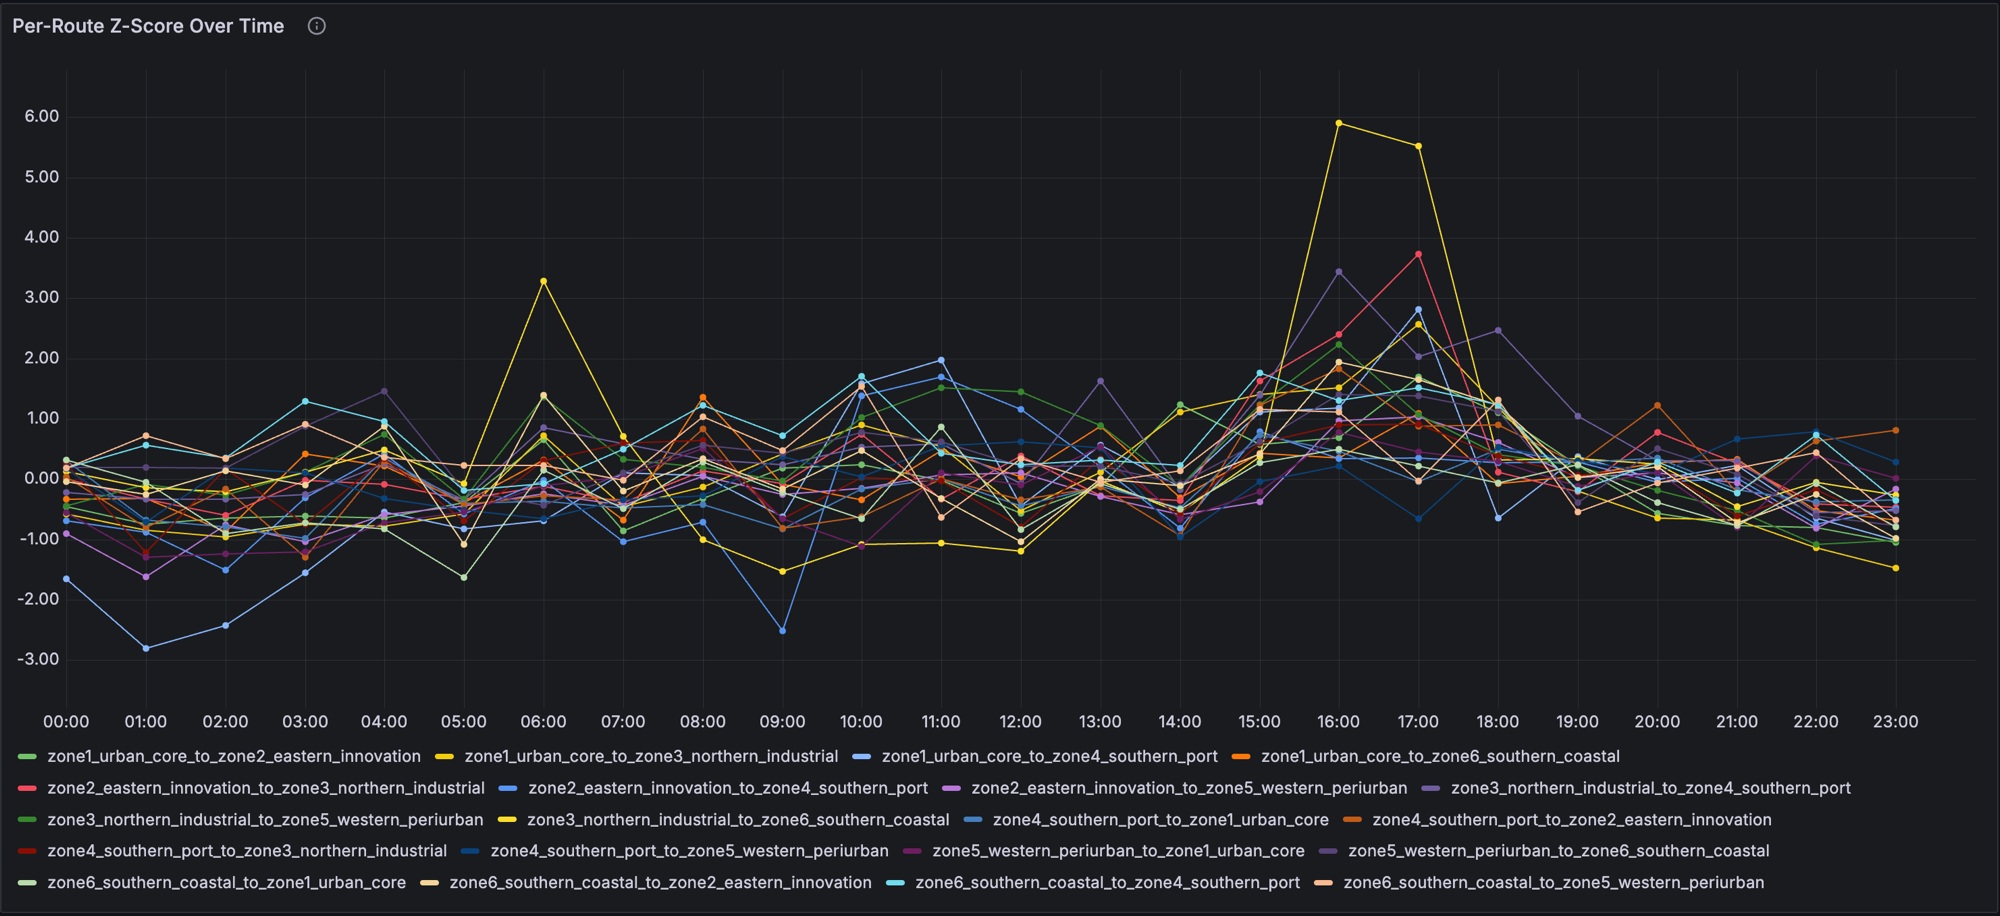
\includegraphics[width=\textwidth]{grafana-zscore-timeseries}
      \caption{Per-route Z-score over a 24-hour observation window
      (Grafana). Each line represents one directed inter-zone route.
      Spikes above the dashed threshold $\theta_r$ trigger the Z-score
      anomaly signal.}
      \label{fig:zscore_timeseries}
  \end{figure}

  % ------------------------------------------------------------
  \subsection{Signal 2 — Isolation Forest Batch Detector}                                                                                                 
  \label{subsec:iforest}
  % ------------------------------------------------------------

  \paragraph{Rationale and Role.}
  The dual-signal framework requires a second, independent detector to reconcile high-recall Z-score signals with high-precision multivariate outlier detection. Isolation Forest \cite{liu2008isolation} is well-suited for this role: it operates on a 7-dimensional feature space (congestion ratios + cyclical time encodings) without requiring labelled data or strong distributional assumptions, and its linear complexity in sample count enables 6-hourly retraining on homelab hardware \cite{isolation_survey_2025}.

  \paragraph{Input, Configuration, Output.}
  The feature vector per route-hour observation comprises three traffic metrics (avg heavy ratio, avg moderate ratio, max severe segments) and four cyclical time encodings (sine-cosine pairs for hour-of-day and day-of-week to ensure temporal circularity). An Isolation Forest model is trained every 6 hours on the Gold-layer corpus ($N \approx 1{,}600$ records per route) using Optuna Bayesian search to maximize the anomaly score gap.
                                                                                                                                                          
  \begin{equation}
  \label{eq:feature_vector}
  \mathbf{x} = (h_{\text{avg}}, m_{\text{avg}}, s_{\text{max}}, \sin(2\pi \cdot \text{hr}/24), \cos(2\pi \cdot \text{hr}/24), \sin(2\pi \cdot \text{dow}/7), \cos(2\pi \cdot \text{dow}/7))
  \end{equation}

  The cyclical encodings (sine-cosine pairs) ensure temporal circularity: hour 23 and hour 0 are geometrically adjacent, preventing false ordinal distances that would mislead the model about traffic periodicity.

  Table~\ref{tab:iforest_params} reports the resulting configuration.
  The \texttt{contamination} value of $0.01$ is consistent with an
  independent heavy-ratio Z-score anomaly rate estimate of $1.97\%$
  obtained by applying the statistical baseline rule to the same training
  corpus, providing cross-signal validation that
  genuine anomalous hours are rare in the pre-cutoff dataset.

  \begin{table}[htbp]
  \centering
  \caption{IsolationForest hyperparameters selected by Optuna TPE
           (50 trials $\times$ 20 routes; median aggregation).}
  \label{tab:iforest_params}
  \begin{tabular}{llll}
  \hline
  \textbf{Parameter} & \textbf{Search range} & \textbf{Default} & \textbf{Tuned} \\
  \hline
  \texttt{contamination} & $[0.01,\;0.15]$ & $0.05$ & $0.01$ \\
  \texttt{n\_estimators}  & $\{50,100,\ldots,500\}$ & $100$ & $450$ \\
  \texttt{max\_samples}   & $[0.5,\;1.0]$  & auto (${\approx}0.17$) & $0.76$ \\
  \texttt{max\_features}  & $[0.5,\;1.0]$  & $1.0$ & $0.73$ \\
  \hline
  \multicolumn{4}{l}{Mean score gap: default $0.059$ $\to$ tuned $0.083$
                     (+40.7\%, 20/20 routes improved).} \\
  \hline
  \end{tabular}
  \end{table}

  Figure~\ref{fig:optuna_validation} validates the tuned parameters against
  the default configuration across all 20 routes.
  The left panel plots tuned score gap against default score gap per route;
  all points lie above the diagonal, confirming improvement on every route.
  The right panel shows the distribution of score gap improvements
  (\texttt{tuned} $-$ \texttt{default}), with all values strictly positive
  (range $+0.01$ to $+0.047$, mean $+0.023$).

  \begin{figure}[htbp]
      \centering
      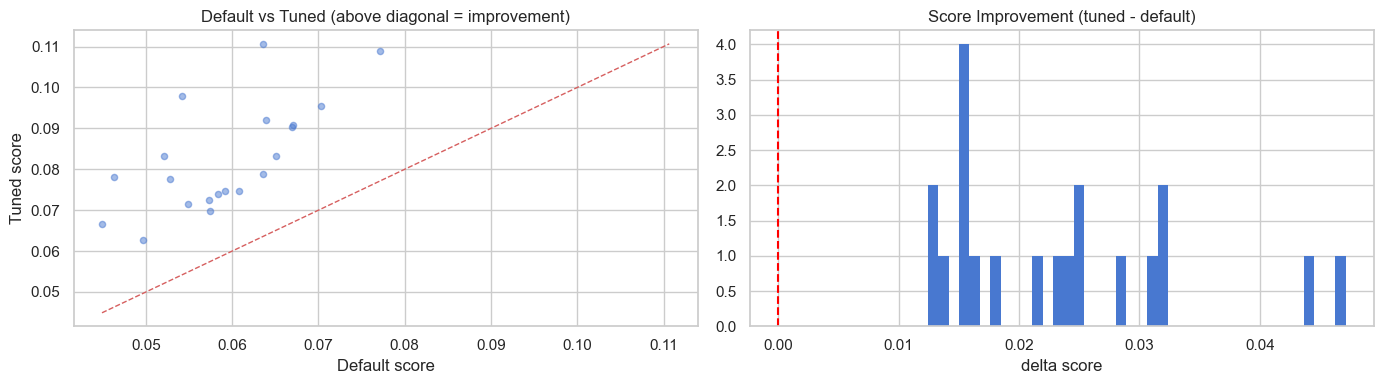
\includegraphics[width=\textwidth]{optuna-validation}
      \caption{Optuna hyperparameter tuning validation across 20 routes.
      \textit{Left}: tuned vs.\ default anomaly score gap per route
      (all points above the diagonal indicate improvement).
      \textit{Right}: distribution of score gap delta
      (\texttt{tuned} $-$ \texttt{default}); all 20 routes show
      strictly positive improvement (mean $+0.023$, max $+0.047$).}
      \label{fig:optuna_validation}
  \end{figure}

  A lower \texttt{contamination} value raises the decision threshold,
  flagging only extreme outliers and biasing the detector towards
  precision; since dual-signal fusion (Section~\ref{subsec:fusion})
  handles recall via Z-score, IForest is tuned for
  high-confidence predictions. Every 6 hours, the model is retrained,
  registered in MLflow with the \texttt{@champion} alias, and loaded
  by the serving layer with a one-hour cache TTL.

  \begin{figure}[htbp]
      \centering
      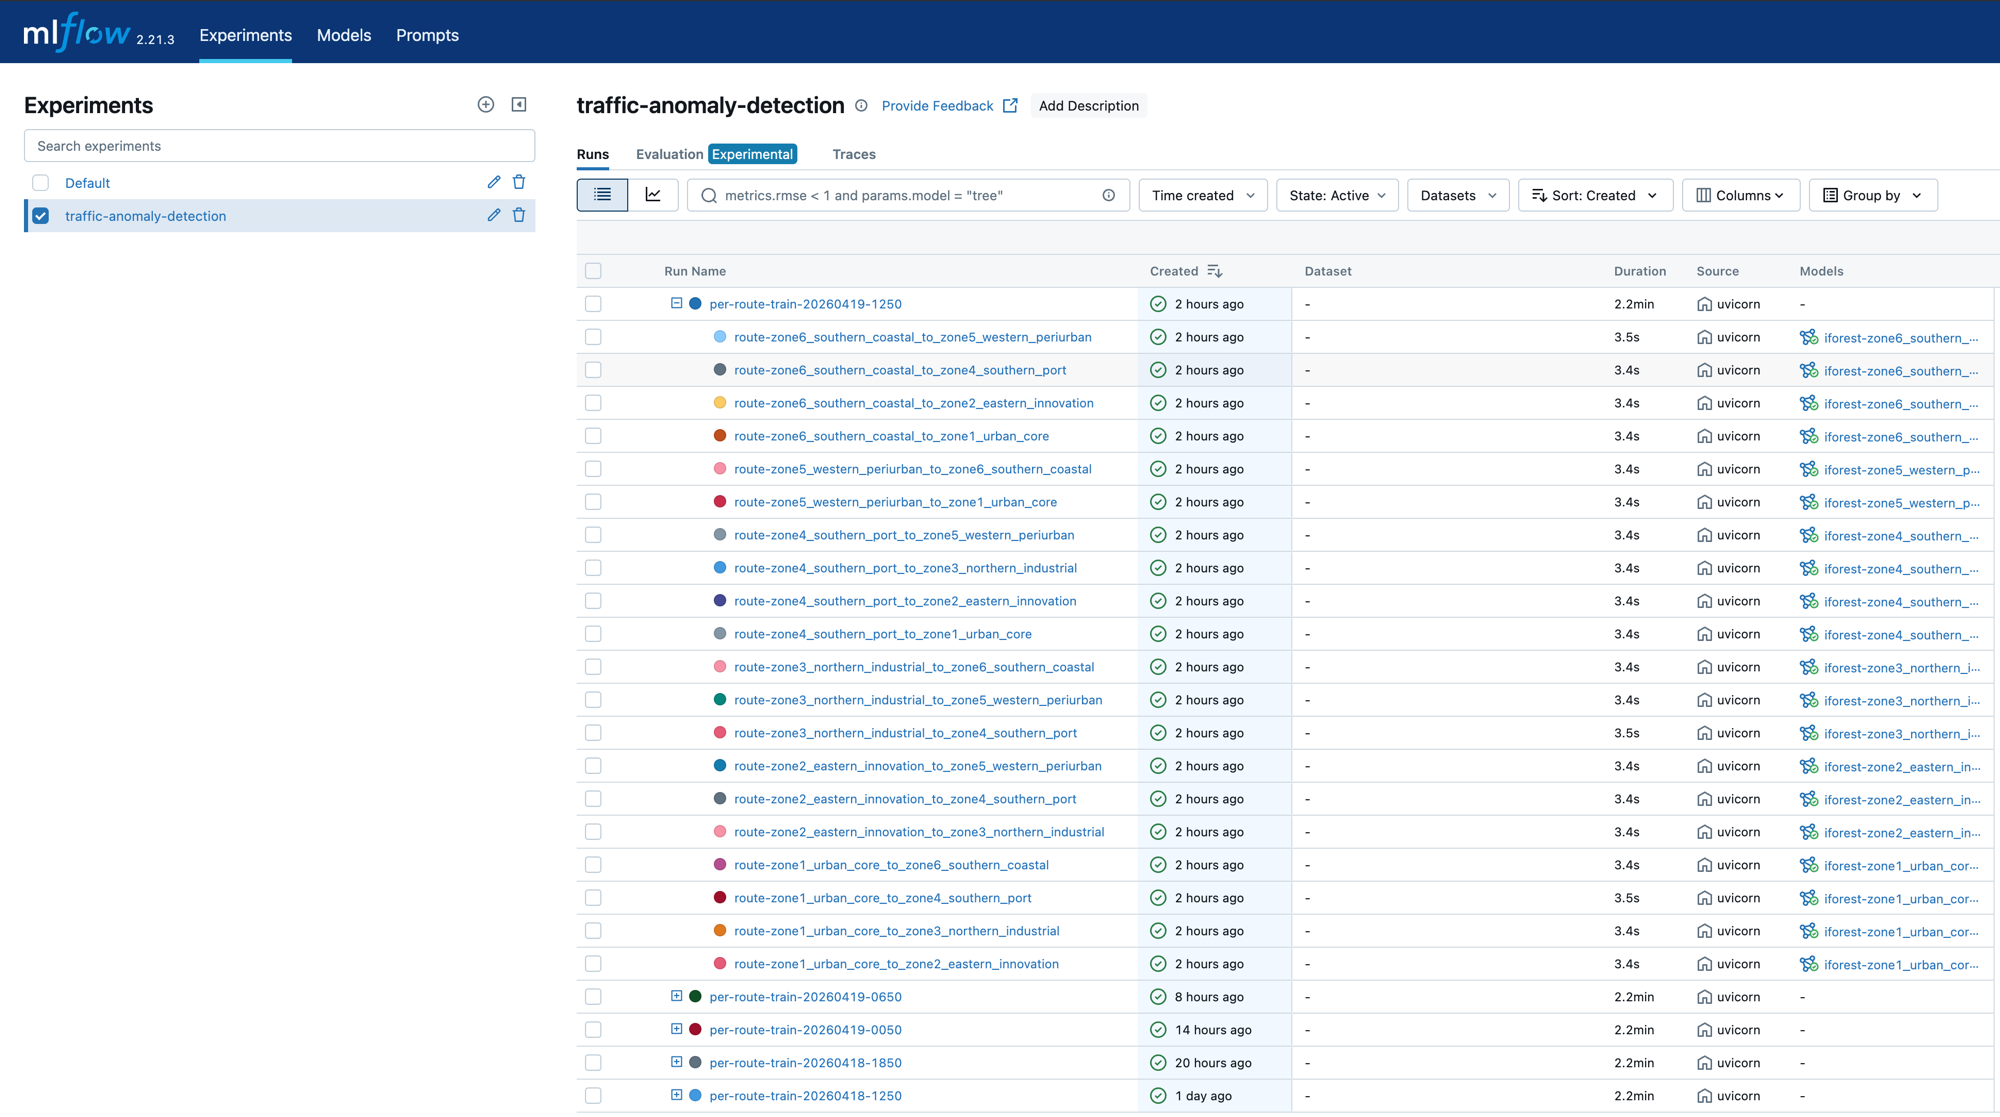
\includegraphics[width=\textwidth]{mlflow-experiments}
      \caption{MLflow experiment view showing per-route
      \texttt{IsolationForest} training runs for the
      \texttt{traffic-anomaly-detection} experiment.
      Each row corresponds to one directed inter-zone route model.}
      \label{fig:mlflow_experiments}
  \end{figure}


  % ------------------------------------------------------------
  \subsection{Dual-Signal Fusion}
  \label{subsec:fusion}                                                                                                                                   
  % ------------------------------------------------------------
                                                                                                                                                          
  The two signals are merged at the Serving Layer into a                                                                                                  
  \textbf{three-tier confidence hierarchy}. Let
  $z_r \in \{0, 1\}$ denote the Z-score anomaly label and                                                                                                 
  $f_r \in \{0, 1\}$ the IsolationForest anomaly label for                                                                                                
  route $r$. The fusion mapping is defined in                                                                                                             
  Algorithm~\ref{alg:fusion}.                                                                                                                             
                                                                                                                                                          
  \begin{algorithm}[H]
      \small                                                                                                                                              
      \caption{$\texttt{tier}_r \gets
      \texttt{SignalFusion}(z_r,\; f_r)$}
      \label{alg:fusion}                                                                                                                                  
      \begin{algorithmic}[1]
          \Require $z_r \in \{0, 1\}$ is the Z-score anomaly label.                                                                                       
          \Require $f_r \in \{0, 1\}$ is the IForest anomaly label.                                                                                       
          \If{$z_r = 1$ \textbf{and} $f_r = 1$}
              \State \Return \textbf{Tier 1}: \texttt{both\_anomaly}                                                                                      
              \Comment{Cross-validated; highest confidence}                                                                                               
          \ElsIf{$z_r = 1$ \textbf{and} $f_r = 0$}                                                                                                        
              \State \Return \textbf{Tier 2}: \texttt{zscore\_anomaly}                                                                                    
              \Comment{Immediate spike; may be transient}                                                                                                 
          \ElsIf{$z_r = 0$ \textbf{and} $f_r = 1$}
              \State \Return \textbf{Tier 3}: \texttt{iforest\_anomaly}                                                                                   
              \Comment{Multivariate pattern; not threshold-detectable}                                                                                    
          \Else
              \State \Return \textbf{Normal}                                                                                                              
          \EndIf                                                                                                                                          
      \end{algorithmic}
  \end{algorithm}                                                                                                                                         
                  
  Automated Telegram alerts are issued only for Tier 1 and Tier 3                                                                                         
  signals, filtered through a \textbf{30-minute per-route cooldown}
  managed in the \texttt{anomaly\_alert\_log} table. This threshold                                                                                       
  suppresses duplicate notifications during sustained congestion                                                                                          
  events whilst ensuring that any new independent anomaly episode                                                                                         
  triggers a fresh alert.                                                                                                                                 
                                                                                                                                                          
  % ============================================================                                                                                          
  \section{Knowledge-Enriched Inference via RAG}
  \label{sec:rag}                                                                                                                                         
  % ============================================================
                                                                                                                                                          
    The anomaly detectors in Section~\ref{sec:anomaly} output reliable
    numerical signals (Z-score and Isolation Forest labels), but those
    outputs alone are not sufficient for operational decision-making.
    Traffic operators need an explanation of \textit{why} congestion is
    occurring, not only whether an anomaly exists. UrbanPulse therefore
    applies \textbf{Retrieval-Augmented Generation (RAG)} \cite{lewis2020rag}
    as an interpretation layer that converts dual-signal alerts into
    root-cause narratives grounded in historical traffic behaviour and
    current weather context.

    % ------------------------------------------------------------
    \subsection{Role in the System (Why)}
    \label{subsec:vector_store}
    % ------------------------------------------------------------

    The role of RAG in UrbanPulse is strictly application-facing:
    \textbf{transforming raw anomaly alerts into actionable knowledge}.
    When an event is flagged, the system should answer a practical
    question for city operators: \textit{why is this route congested now?}
    In many cases, the explanation is compositional (for example, an
    unusual congestion spike coinciding with adverse weather during a
    peak-hour corridor). RAG is used to synthesise this multi-source
    context into concise natural language that can be consumed directly in
    dashboard workflows.

    % ------------------------------------------------------------
    \subsection{Implementation Pipeline (Input -- Configuration -- Output)}
    \label{subsec:rag_indexing}
    % ------------------------------------------------------------

    UrbanPulse implements RAG as a black-box inference pipeline with three
    operational stages:

    \begin{enumerate}
      \item \textbf{Input (Retrieval):} RAG is triggered for
      high-confidence events where both detection signals agree
      (\texttt{both\_anomaly}). The serving layer retrieves traffic
      context from ChromaDB (recent anomaly events and historical route
      patterns) and, in parallel, fetches current meteorological context
      from Open-Meteo.

      \item \textbf{Configuration (Model and Prompting):} Generation is
      executed by a local \textbf{Qwen2.5:3b} model served via
      \textbf{Ollama} \cite{qwen25_report,ollama_docs}. The local-LLM
      deployment is a deliberate infrastructure decision motivated by
      three constraints: municipal data privacy, predictable operating
      cost (no per-token external billing), and offline-capable
      deployment on city-controlled infrastructure. Retrieved traffic
      evidence and live weather variables are injected into a fixed prompt
      template together with numerical anomaly indicators
      (e.g., Z-score magnitude, congestion ratios, and route metadata).

      \item \textbf{Output (Generation):} The LLM returns a concise
      root-cause explanation in natural language, streamed via
      \textbf{Server-Sent Events} (SSE) \cite{sse_spec} and rendered
      directly in the operator interface (Grafana/UI) alongside the alert.
    \end{enumerate}

    This implementation is intentionally concise: from anomaly trigger to
    human-readable explanation in a single retrieval-augmentation-generation
    flow, without additional iterative reasoning loops in the serving path.
                                                                                                                                                          
  % ------------------------------------------------------------
  \subsection{Feedback Loop and Fine-Tuning Data Collection}                                                                                              
  \label{subsec:feedback}
  % ------------------------------------------------------------

  Every LLM interaction — query string, retrieved chunks with                                                                                             
  similarity scores, and the full generated response — is persisted
  to the \texttt{rag\_interaction\_log} PostgreSQL table. The                                                                                             
  \texttt{/rca/feedback} endpoint accepts a thumbs-up ($+1$) or                                                                                           
  thumbs-down ($-1$) rating per interaction, stored in the                                                                                                
  \texttt{feedback} column. This produces a continuously growing,                                                                                         
  human-labelled dataset suitable for future \textit{supervised                                                                                           
  fine-tuning} of the retrieval ranking or generation components                                                                                          
  \cite{rlhf_paper}, distinguishing UrbanPulse from systems that                                                                                          
  treat the LLM as a stateless inference endpoint.                                                                                                        
                                                                                                                                                          
  % ============================================================                                                                                          
  \section{Evaluation Framework}                                                                                                                          
  \label{sec:evaluation}                                                                                                                                  
  % ============================================================
                                                                                                                                                          
  The methodologies described in the preceding sections are designed                                                                                      
  to satisfy the three operational pillars established in
  Section~\ref{sec:requirements}: \textit{temporal integrity},                                                                                            
  \textit{reproducibility}, and \textit{observability}. This section                                                                                      
  defines the specific metrics and measurement boundaries that                                                                                            
  Chapter~4 will report.                                                                                                                                  

  \paragraph{Experimental Protocol.}
  The empirical evaluation follows a fixed protocol to ensure repeatable and comparable results. Traffic telemetry is collected continuously over a bounded observation window and retained at Bronze, Silver, Gold, and online-feature granularity. All experiments are executed on a single, fixed deployment environment; the hardware profile (CPU, memory, GPU, storage) and software stack (Docker, Python, Redpanda, PostgreSQL, MinIO, Iceberg/Nessie, MLflow, ChromaDB, Ollama) are recorded before each evaluation run.

  The workload profile consists of three measurement modes: (i) normal-load run using production polling and all routes, (ii) stress run replaying messages at $2\times$ throughput to assess stability, and (iii) inference run issuing repeated requests to measure latency under steady-state conditions. Baseline comparison is performed against a batch-only variant where anomaly labels become available only after periodic aggregation. For each metric, measurements are computed from persisted logs or monitoring systems using $p_{50}$, $p_{95}$, and max statistics.

  % ============================================================
  \subsection{Temporal Integrity}
  \label{subsec:eval_temporal}
  % ============================================================

  All Bronze Parquet files are partitioned by event timestamp.                                                                                            
  End-to-end ingestion lag $L_{\text{e2e}}$ is defined as:
                                                                                                                                                          
  \begin{equation}
  \label{eq:lag}                                                                                                                                          
  L_{\text{e2e}}^{(r,t)} = t_{\text{feature}} - t_{\text{ingest\_ts}}
  \end{equation}                                                                                                                                          
   
  where $t_{\text{ingest\_ts}}$ is the Unix millisecond timestamp                                                                                         
  recorded immediately before the VietMap API call (embedded in the
  Kafka message header) and $t_{\text{feature}}$ is the time at which                                                                                     
  the corresponding \texttt{UPSERT} completes in PostgreSQL. This metric
  is exposed per-route and aggregated at \texttt{/online/lag} as                                                                                          
  $p_{50}$, $p_{95}$, and $\max$. The target for NFR-1 is                                                                                                 
  $L_{\text{e2e}}^{p_{95}} < 20\,\text{s}$.                                                                                                               
                                                                                                                                                          
  % ------------------------------------------------------------                                                                                          
  \subsection{Reproducibility}                                                                                                                            
  \label{subsec:eval_reproducibility}
  % ------------------------------------------------------------

  Two mechanisms jointly ensure reproducibility. First, the                                                                                               
  \textbf{Apache Iceberg} time-travel API allows any Silver or
  Gold table to be queried at any historical snapshot by ID                                                                                               
  or timestamp — meaning the exact data state at the time of
  any anomaly classification can be reconstructed. Second,                                                                                                
  \textbf{MLflow} records the full provenance of every
  IsolationForest training run: hyperparameters
  (\texttt{contamination}, \texttt{n\_estimators},
  \texttt{max\_samples}, \texttt{max\_features},
  \texttt{random\_state}, \texttt{training\_cutoff}),
  feature schema, and training data time
  range; therefore, each inference can be replayed against the same
  model version and data snapshot.                                                                                                                                          
                                                                                                                                                          
  % ------------------------------------------------------------                                                                                          
\subsection{Performance Metrics}
  \label{subsec:performance_metrics}
  % ------------------------------------------------------------
                
  The following metrics summarise the system's ability to satisfy the operational pillars:
            
  \begin{table}[h]
  \centering
  \caption{Performance metrics: temporal integrity, reproducibility, and system performance}
  \label{tab:performance_metrics}
  \resizebox{\textwidth}{!}{%
  \begin{tabular}{llll}
  \hline               
  \textbf{KPI} & \textbf{Definition} & \textbf{Target} &                                                                                                  
  \textbf{Measurement point} \\                         
  \hline                                                                                                                                                  
  Ingestion lag $p_{95}$    & $t_{\text{feature}} - t_{\text{ingest\_ts}}$
                            & $< 20\,\text{s}$                                                                                                            
                            & \texttt{/online/lag} \\                                                                                                     
  Microbatch freshness      & Bronze write $\to$ Silver commit
                            & $< 5\,\text{min}$                                                                                                           
                            & Prefect task duration \\                                                                                                    
  IForest scoring latency   & Background scorer cycle
                              duration (15\,s interval)
                            & $< 5\,\text{s}$
                            & Serving API logs \\                                                                                                         
  \hline                                                                                                                                                  
  \end{tabular}
  }%
  \end{table}                                                                                                                                             
                                                                                                                                                          
  By integrating periodic high-velocity API polling with an incrementally
  processed, versioned Data Lakehouse and two independent, orthogonal                                                                                     
  anomaly detectors, the methodology presented in this chapter provides
  a rigorous foundation for evaluating UrbanPulse's ability to maintain                                                                                   
  low-latency, reproducible situational awareness under real-world                                                                                        
  metropolitan workloads in Ho Chi Minh City.                                                                                                             
                                                                                                                                                          
 


\chapter{PROTOTYPING}
This chapter documents the prototyping phase of the UrbanPulse platform, covering
the technology selection rationale, containerised infrastructure design, core data
schema decisions, and the incremental validation strategy used before full
implementation began.

% ============================================================
\section{Technology Stack Selection}
\label{sec:tech-selection}
% ============================================================

The UrbanPulse prototype is built on a curated stack of open-source components.
Each technology was evaluated against three criteria: \textit{(i)} compatibility
with Python 3.12 and the \texttt{uv} monorepo toolchain, \textit{(ii)} support
for streaming-first workloads, and \textit{(iii)} availability as a
self-hostable Docker image suitable for homelab deployment.
Table~\ref{tab:tech-stack} summarises the chosen components and their roles.

\begin{table}[htbp]
\centering
\caption{UrbanPulse technology stack and selection rationale.}
\label{tab:tech-stack}
\resizebox{\textwidth}{!}{%
\begin{tabular}{llll}
\hline
\textbf{Component} & \textbf{Technology} & \textbf{Version} & \textbf{Rationale} \\
\hline
Message Broker     & Redpanda            & v25.3.10 & Kafka-compatible; no ZooKeeper; lower memory \\
Object Storage     & MinIO               & latest   & S3-compatible API; local deployment \\
Table Format       & Apache Iceberg      & 0.9.x    & Schema evolution; time-travel; partition pruning \\
Catalog            & Project Nessie      & 0.99.0   & Git-like branching; REST API \\
Online Store       & PostgreSQL          & 15       & UPSERT semantics; asyncpg for async serving \\
Vector Store       & ChromaDB            & 0.4.x    & Embedded; nomic-embed compatible \\
Orchestration      & Prefect             & 3.x      & Task retries; flow scheduling; UI dashboard \\
ML Tracking        & MLflow              & 2.21.3   & Experiment logging; model registry \\
LLM Runtime        & Ollama              & latest   & Local GPU inference; Qwen2.5:3b \\
Serving            & FastAPI             & 0.115.x  & Async; SSE support; Pydantic v2 \\
Reverse Proxy      & Traefik             & v3       & Automatic TLS; label-based routing \\
Monitoring         & Grafana + Loki      & latest   & Log aggregation; dashboard \\
Frontend           & Next.js 15 + TypeScript & 15   & App Router; real-time SSE client \\
\hline
\end{tabular}%
}
\end{table}

\subsection{Message Broker: Redpanda over Apache Kafka}

\textbf{Redpanda}~\cite{redpanda_whitepaper} was selected over vanilla Apache
Kafka for two practical reasons. First, Redpanda eliminates the ZooKeeper
dependency, reducing the container count by two services. Second, its
\textit{single-binary} architecture yields lower memory consumption, which
is critical for the homelab Intel~i5 deployment environment. The Kafka-wire
compatibility ensures that all \texttt{confluent\_kafka} Python clients work
without modification.

\subsection{Storage: Iceberg + Nessie + MinIO}

Raw Parquet files in MinIO constitute the \textbf{Bronze layer}. Promoting
data to \textbf{Silver} and \textbf{Gold} requires a table format that
supports (a) transactional writes from micro-batches, (b) schema evolution
without full rewrites, and (c) time-travel for reprocessing. \textbf{Apache
Iceberg}~\cite{iceberg_paper} satisfies all three. \textbf{Project
Nessie}~\cite{nessie_docs} provides the REST catalog, enabling branching and
atomic commits without locking MinIO objects directly.

\subsection{LLM: Ollama with Qwen2.5:3b}

The RAG pipeline requires a model that fits within the homelab GPU budget
(NVIDIA GTX~1060, 6~GB VRAM). \textbf{Qwen2.5:3b}~\cite{qwen25_report},
served via \textbf{Ollama}, achieves an average time-to-first-token of under
one second while producing coherent 2--3 sentence traffic explanations in
both English and Vietnamese. The \textit{RAG-over-fine-tuning} approach is
justified by the need for always-current context: retraining on new anomaly
events would be prohibitively expensive on the available hardware.

% ============================================================
\section{Service Topology Design}
\label{sec:topology}
% ============================================================

The platform is decomposed into \textbf{six microservices}, each running as an
independent Docker container. Services communicate exclusively through two
channels: the \textbf{Redpanda broker} (event streams) and
\textbf{PostgreSQL} (materialised feature store). No direct service-to-service
HTTP calls exist in the hot path, ensuring fault isolation.

Figure~\ref{fig:service-topology} illustrates the container topology and the
two communication channels.

\begin{figure}[htbp]
\centering
\resizebox{0.92\textwidth}{!}{%
\begin{tikzpicture}[
  >=stealth, font=\small,
  svc/.style={draw, rounded corners=4pt, fill=white,
              minimum width=3.0cm, minimum height=0.9cm,
              align=center, font=\footnotesize, inner sep=5pt},
  infra/.style={draw, rounded corners=4pt, fill=gray!10,
                minimum width=3.0cm, minimum height=0.9cm,
                align=center, font=\footnotesize, inner sep=5pt},
  karr/.style={->, thick, blue!60},
  parr/.style={->, thick, green!50!black},
  harr/.style={->, thick, orange!80!black},
  lbl/.style={font=\scriptsize}
]

%% Infrastructure layer (bottom band)
\fill[gray!8, rounded corners=5pt] (-7.5,-1.2) rectangle (7.5,1.2);
\node[font=\scriptsize\itshape] at (0,1.0) {Infrastructure Layer};
\node[infra] (redpanda) at (-4.5, 0) {Redpanda\\(Kafka broker)};
\node[infra] (postgres) at (0,    0) {PostgreSQL\\(Feature store)};
\node[infra] (minio)    at (4.5,  0) {MinIO\\(Object store)};

%% Application services (top)
\node[svc] (ingest)    at (-6.0,  3.2) {Ingestion\\Service};
\node[svc] (streaming) at (-2.5,  3.2) {Streaming\\Service};
\node[svc] (online)    at ( 0.8,  3.2) {Online\\Service};
\node[svc] (batch)     at ( 3.5,  3.2) {Batch\\Service};
\node[svc] (ml)        at ( 6.0,  3.2) {ML\\Service};
\node[svc] (serving)   at ( 0.0,  5.2) {Serving\\(FastAPI)};

%% Ingest → Redpanda
\draw[karr] (ingest.south) -- ++(0,-0.6) -| (redpanda.north);

%% Redpanda → Streaming, Online
\draw[karr] (redpanda.north) -- ++(0,0.5) -| (streaming.south);
\draw[karr] (redpanda.north) -- ++(0,0.5) -| (online.south);

%% Streaming → MinIO
\draw[->, thick, purple!60] (streaming.east) -- ++(0.4,0) |- (minio.north);

%% Online → PostgreSQL
\draw[parr] (online.south) -- ++(0,-0.5) -| (postgres.north);

%% Batch → MinIO (read/write) + PostgreSQL (write baseline)
\draw[->, thick, purple!60] (batch.south) -- ++(0,-0.4) -| (minio.north);
\draw[parr] (batch.south)   -- ++(0,-0.4) -| (postgres.north);

%% ML ↔ MLflow (external, simplified as arrow to batch)
\draw[harr, dashed] (ml.west) -- (batch.east) node[midway, above, lbl] {POST /train};

%% Serving ← PostgreSQL + MinIO
\draw[parr] (postgres.north) -- ++(0,1.0) -| (serving.south);
\draw[->, thick, purple!60] (minio.north) -- ++(0,0.6) -| (serving.south);

%% Legend
\node[lbl, blue!60]            at (-5.8,-0.8)  {--- Kafka};
\node[lbl, green!50!black]     at (-3.8,-0.8)  {--- PostgreSQL};
\node[lbl, purple!60]          at (-1.8,-0.8)  {--- MinIO/S3};
\node[lbl, orange!80!black]    at ( 0.6,-0.8)  {- - HTTP};

\end{tikzpicture}%
}
\caption{UrbanPulse service topology: six microservices communicating via
         Redpanda (blue) and PostgreSQL (green). Dashed orange indicates the
         HTTP trigger from Batch to ML service.}
\label{fig:service-topology}
\end{figure}

% ============================================================
\section{Data Schema Design}
\label{sec:schema-design}
% ============================================================

\subsection{Kafka Message Schema}

Every traffic observation published to Redpanda is serialised as JSON conforming
to the \texttt{TrafficRouteObservation} Pydantic model. The canonical fields are:

\begin{itemize}
  \item \textbf{\texttt{route\_id}}: unique string identifier of the inter-zone
        route (e.g., \texttt{zone1\_urban\_core\_\allowbreak to\_zone2\_eastern\_innovation}).
  \item \textbf{\texttt{duration\_ms}}: raw travel time from the VietMap Directions
        API, in milliseconds.
  \item \textbf{\texttt{duration\_minutes}}: derived field ($= \texttt{duration\_ms}
        / 60000$), rounded to one decimal place.
  \item \textbf{\texttt{congestion}}: nested object containing
        \texttt{heavy\_ratio}, \texttt{moderate\_ratio},
        \texttt{low\_ratio} (each a fraction $[0,1]$),
        \texttt{severe\_segments} (integer count), and
        \texttt{total\_segments}.
  \item \textbf{\texttt{timestamp\_utc}}: ISO-8601 timestamp at which the API
        was polled.
\end{itemize}

\noindent A Kafka header \texttt{ingest\_ts} (Unix milliseconds) is attached at
publish time to enable end-to-end ingestion lag measurement in the Online Service.

\subsection{Iceberg Table Schemas}

Three Iceberg tables are provisioned in MinIO via Nessie catalog:

\begin{enumerate}
  \item \textbf{Silver} (\texttt{silver.traffic\_route}): 13-column schema
        with one row per API observation. Partitioned by \texttt{day(timestamp\_utc)}.
        A \texttt{source} column records the VietMap API endpoint version.
  \item \textbf{Gold} (\texttt{gold.traffic\_hourly}): 11-column hourly
        aggregation keyed by \texttt{(route\_id, hour\_utc)}. Includes
        \texttt{avg\_heavy\_ratio}, \texttt{avg\_moderate\_ratio},
        \texttt{avg\_duration\_minutes}, and \texttt{p95\_duration\_minutes}.
        Partitioned by \texttt{day(hour\_utc)}.
  \item \textbf{Baseline} (\texttt{gold.traffic\_baseline}): per-route,
        per-hour-of-day, per-day-of-week statistical summary used by the
        Online Service Z-score computation.
\end{enumerate}

\subsection{PostgreSQL Online Store}

The table \texttt{online\_route\_features} persists the current hourly window
state for every route, with primary key \texttt{(route\_id, window\_start)}.
It serves two purposes: (a) it is the low-latency read target of the Serving
API, and (b) it acts as a crash-recovery checkpoint --- on restart, the Online
Service reconstructs Welford accumulators from stored
\texttt{mean} and \texttt{stddev} values via the identity
$M_2 = \sigma^2 \times (n - 1)$.

% ============================================================
\section{Infrastructure Prototyping}
\label{sec:infra-proto}
% ============================================================

The entire platform is containerised using \textbf{Docker Compose} with a
three-file layered override pattern:

\begin{itemize}
  \item \texttt{docker-compose\allowbreak.base.yaml} --- shared service definitions
        (Redpanda, MinIO, Nessie, PostgreSQL, ChromaDB, MLflow, Prefect, Ollama).
  \item \texttt{docker-compose\allowbreak.dev.yaml} --- development overlay: exposes ports
        locally, mounts source code volumes, uses \texttt{host.docker.internal}
        for the Ollama endpoint.
  \item \texttt{docker-compose\allowbreak.prod.yaml} --- production overlay: adds
        Traefik reverse proxy with Let's Encrypt TLS, removes exposed ports,
        uses named volumes at \texttt{/opt/urban-pulse/} on the host.
\end{itemize}

\noindent The \texttt{Makefile} provides validated entry points (\texttt{make dev},
\texttt{make prod}, \texttt{make bootstrap}, \texttt{make train}) so that the
multi-container stack can be brought up or torn down deterministically. The
\texttt{bootstrap} target seeds Redpanda topics, MinIO buckets, and Prefect
deployment schedules in a single pass before live traffic is processed.


\chapter{IMPLEMENTATION}
This chapter details the implementation of each UrbanPulse microservice, tracing
the data path from raw API polling through streaming ingestion, lakehouse
persistence, machine learning inference, and finally the serving layer that
delivers results to the frontend.

% ============================================================
\section{Ingestion Service}
\label{sec:impl-ingestion}
% ============================================================

The \textbf{Ingestion Service} is a long-running Python process that polls the
\textbf{VietMap Directions API} every \textbf{5 minutes} for 20 predefined
inter-zone routes across Ho Chi Minh City. Each route is defined by an origin
and destination anchor point (WGS-84 latitude/longitude pair) together with
a human-readable zone label.

\subsection{VietMap API Integration}

The \texttt{sources/vietmap.py} module constructs a REST request to the
\texttt{/api/route/v3} endpoint, requesting \texttt{congestion} annotations
per road segment:

\begin{lstlisting}[language=Python,
  caption={VietMap congestion metric extraction.},
  label={lst:vietmap}]
def _calc_congestion(segments: list[dict]) -> CongestionMetrics:
    total = len(segments)
    counts = {"heavy": 0, "moderate": 0, "low": 0, "severe": 0}
    for seg in segments:
        v = seg.get("value", "")
        if v in counts:
            counts[v] += 1
    return CongestionMetrics(
        heavy_ratio=round(counts["heavy"] / total, 3),
        moderate_ratio=round(counts["moderate"] / total, 3),
        severe_segments=counts["severe"],
        total_segments=total,
    )
\end{lstlisting}

\noindent The resulting \texttt{TrafficRouteObservation} object is serialised to
JSON and published to the Redpanda topic \texttt{traffic-route-bronze} with a
Kafka header \texttt{ingest\_ts} (Unix milliseconds) attached for downstream
lag measurement.

Figure~\ref{fig:redpanda-topic} shows the Redpanda Console confirming
\textbf{67,428 messages} accumulated in the \texttt{traffic-route-bronze}
topic (34.3~MiB) across the 40-day deployment, corresponding to the expected
$20 \text{ routes} \times 288 \text{ polls/day} \times 40 \text{ days} =
230{,}400$ raw messages before compaction.

\begin{figure}[htbp]
  \centering
  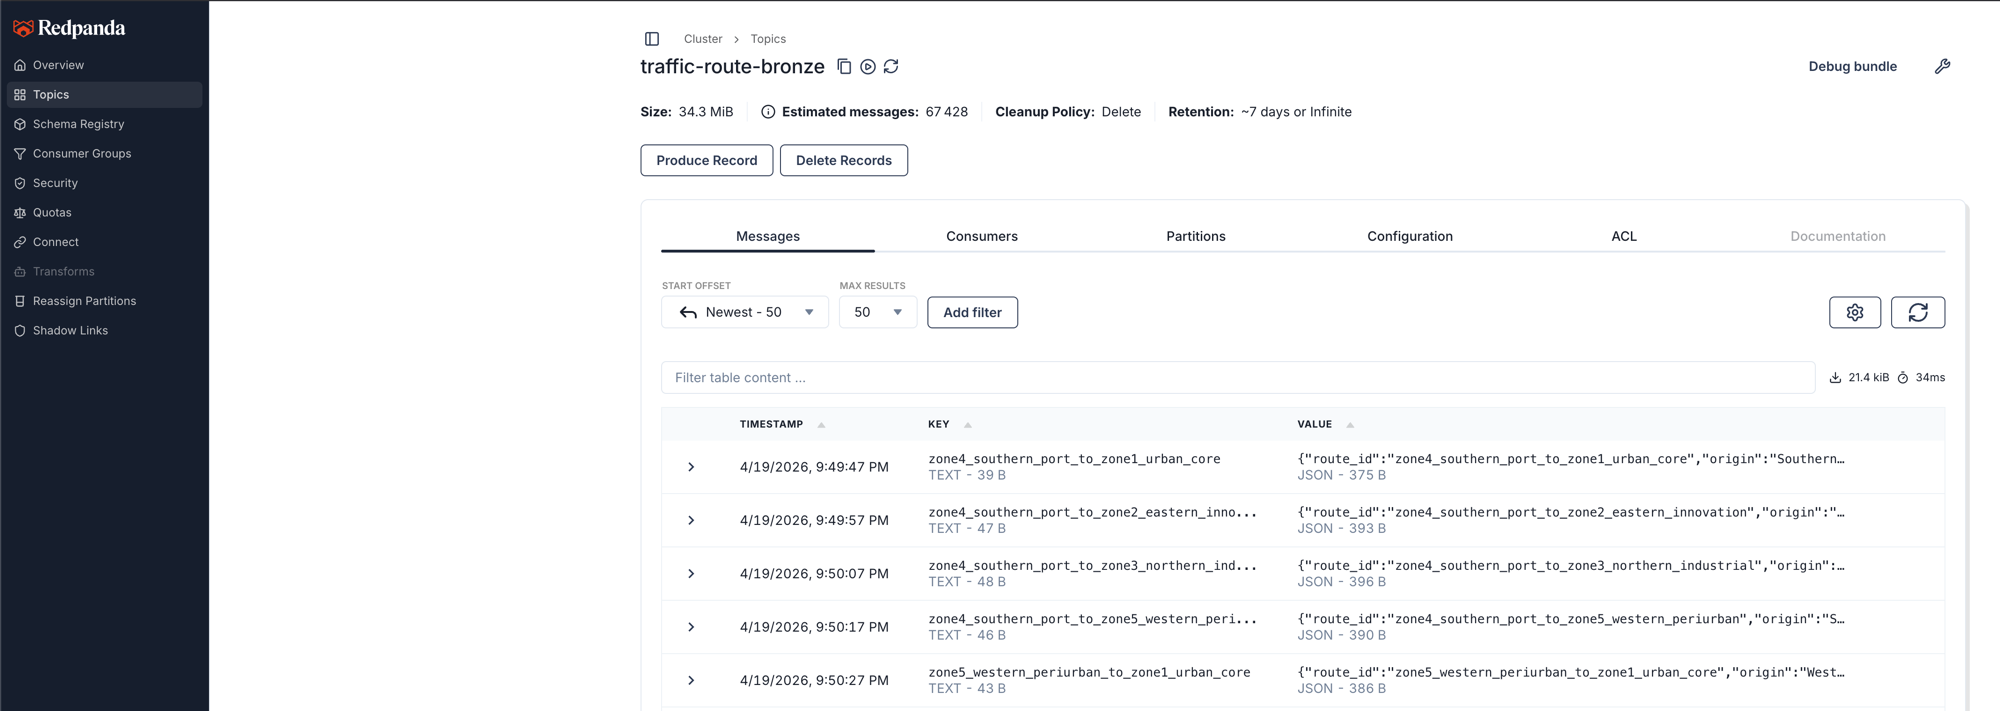
\includegraphics[width=\textwidth]{redpanda-topic.png}
  \caption{Redpanda Console: \texttt{traffic-route-bronze} topic with 67,428
           messages (34.3~MiB) confirming continuous ingestion over the
           40-day observation window.}
  \label{fig:redpanda-topic}
\end{figure}

\subsection{Concurrent Route Polling}

The \texttt{orchestrator.py} module spawns one coroutine per route using
\texttt{asyncio.gather}, so all 20 API calls proceed concurrently within the
5-minute window. Failed requests raise \texttt{HTTPError} and are logged
without crashing the process; the next polling cycle attempts the route again
automatically.

% ============================================================
\section{Streaming Service}
\label{sec:impl-streaming}
% ============================================================

The \textbf{Streaming Service} subscribes to \texttt{traffic\allowbreak-route\allowbreak-bronze}
(consumer group \texttt{streaming\allowbreak-group}) and writes each message as a
Parquet file to MinIO under the time-partitioned path:

\begin{center}
\ttfamily\small
s3://urban-pulse/bronze/traffic-route-bronze/\\
\hspace*{2em}year=\{Y\}/month=\{M\}/day=\{D\}/hour=\{H\}/\{uuid\}.parquet
\end{center}

The processor (\texttt{processors/traffic.py}) deserialises the JSON payload
into a \texttt{TrafficRouteObservation}, converts it to a single-row
\texttt{PyArrow} RecordBatch, and flushes it to MinIO via
\texttt{sinks/minio.py}. This write-once-per-message approach (micro-file
pattern) intentionally creates many small Parquet files; the Batch Service
later compacts them during the Bronze-to-Silver promotion step.

% ============================================================
\section{Online Service}
\label{sec:impl-online}
% ============================================================

The \textbf{Online Service} runs a second consumer group
(\texttt{online-features-group}) on the same topic in parallel with the
Streaming Service, implementing a stateful \textbf{Welford online
algorithm}~\cite{welford1962} for per-route rolling statistics.

\subsection{Welford Accumulator}

For each route, a \texttt{RouteWindow} object maintains the Welford state
$(n, \bar{x}, M_2)$ where $n$ is the observation count, $\bar{x}$ is the
running mean of travel duration, and $M_2 = \sum(x_i - \bar{x})^2$.
On each new observation $x$:

\begin{align}
  n     &\leftarrow n + 1 \\
  \delta &= x - \bar{x} \\
  \bar{x} &\leftarrow \bar{x} + \delta / n \\
  M_2   &\leftarrow M_2 + \delta \cdot (x - \bar{x}) \\
  \sigma &= \sqrt{M_2 / (n - 1)} \quad (n > 1)
\end{align}

\noindent This formulation is numerically stable and requires $O(1)$ memory
regardless of observation history~\cite{welford1962}.

\subsection{Z-Score Anomaly Signal}

After each update, the current window mean \texttt{mean\_heavy\_ratio} is
compared against the route's baseline statistics loaded from the
\texttt{gold.traffic\_baseline} Iceberg table:

\begin{equation}
  Z_{\text{heavy}} = \frac{\bar{r}_\text{window} - \mu_\text{baseline}}
                          {\sigma_\text{baseline}}
\end{equation}

A one-sided threshold $Z > \theta$ (default $\theta = 2.0$, overridden per
route from the baseline's \texttt{zscore\_threshold} column) marks the window
as \texttt{is\_anomaly = TRUE}. The one-sided formulation is intentional:
\textit{low} heavy traffic is never an incident; only elevated congestion
warrants an alert.

\subsection{Crash Recovery}

On restart, the service calls \texttt{\_restore\_windows()} which queries the
current hour's rows from \texttt{online\_route\_features}. The Welford
accumulator is reconstructed from the stored mean and standard deviation using
the algebraic inverse $M_2 = \sigma^2 \times (n - 1)$, allowing the service to
continue accumulating mid-hour without resetting to zero.

% ============================================================
\section{Batch Pipeline}
\label{sec:impl-batch}
% ============================================================

The \textbf{Batch Service} is orchestrated by \textbf{Prefect 3.x} and
executes four distinct flows on separate schedules as shown in
Figure~\ref{fig:batch-flows}.

\begin{figure}[htbp]
\centering
\resizebox{0.88\textwidth}{!}{%
\begin{tikzpicture}[
  >=stealth, font=\small,
  box/.style={draw, rounded corners=3pt, fill=white,
              minimum width=3.8cm, minimum height=0.8cm,
              align=center, font=\footnotesize, inner sep=5pt},
  sched/.style={font=\scriptsize\itshape, gray!60!black},
  arr/.style={->, thick}
]

%% Timeline axis
\draw[thick, ->] (-0.5,0) -- (14.5,0) node[right]{\scriptsize time};

%% Microbatch (every 5 min)
\foreach \x in {0, 1.4, 2.8, 4.2, 5.6, 7.0, 8.4, 9.8, 11.2, 12.6}{
  \fill[blue!25] (\x,-0.15) rectangle (\x+1.0,0.15);
}
\node[sched] at (6.2, 0.55) {every 5 min};
\node[box, fill=blue!12] at (1.7, 1.6) {Bronze → Silver\\(microbatch)};
\draw[arr, blue!60] (1.7,1.15) -- (1.7,0.2);

%% Hourly gold
\foreach \x in {0, 4.2, 8.4, 12.6}{
  \fill[yellow!40] (\x,-0.3) rectangle (\x+4.0,-0.15);
}
\node[sched] at (6.2, -0.65) {every 60 min};
\node[box, fill=yellow!20] at (5.5, -1.6) {Silver → Gold\\+ Baseline learning};
\draw[arr, yellow!60!black] (5.5,-1.15) -- (5.5,-0.35);

%% Retrain (every 6 h)
\foreach \x in {0, 8.4}{
  \fill[red!20] (\x,-0.5) rectangle (\x+8.0,-0.35);
}
\node[sched] at (8.4, -2.45) {every 6 h};
\node[box, fill=red!10] at (9.5, -2.8) {ML Retrain\\+ RAG indexing};
\draw[arr, red!60] (9.5,-2.45) -- (9.5,-0.5);

%% Alerter (every 5 min)
\foreach \x in {0, 1.4, 2.8, 4.2, 5.6, 7.0, 8.4, 9.8, 11.2, 12.6}{
  \fill[green!25] (\x,-0.65) rectangle (\x+1.0,-0.5);
}
\node[sched] at (12.0, 0.55) {every 5 min};
\node[box, fill=green!10] at (12.5, 1.6) {Anomaly Alerter\\(Telegram)};
\draw[arr, green!60!black] (12.5,1.15) -- (12.5,0.2);

\end{tikzpicture}%
}
\caption{Prefect flow schedules: microbatch and alerter run every 5 minutes;
         gold aggregation runs hourly; ML retrain runs every 6 hours.}
\label{fig:batch-flows}
\end{figure}

Figure~\ref{fig:prefect-deployments} shows the Prefect UI confirming all
seven production deployments are active: \texttt{alert\allowbreak-check} and
\texttt{traffic\allowbreak-microbatch} run every 5 minutes,
\texttt{hourly\allowbreak-gold\allowbreak-run} runs hourly,
\texttt{traffic\allowbreak-retrain} and \texttt{rag\allowbreak-index\allowbreak-rebuild}
run every 6 hours, and \texttt{backfill\allowbreak-silver} and
\texttt{bootstrap\allowbreak-infra} run on-demand.

\begin{figure}[htbp]
  \centering
  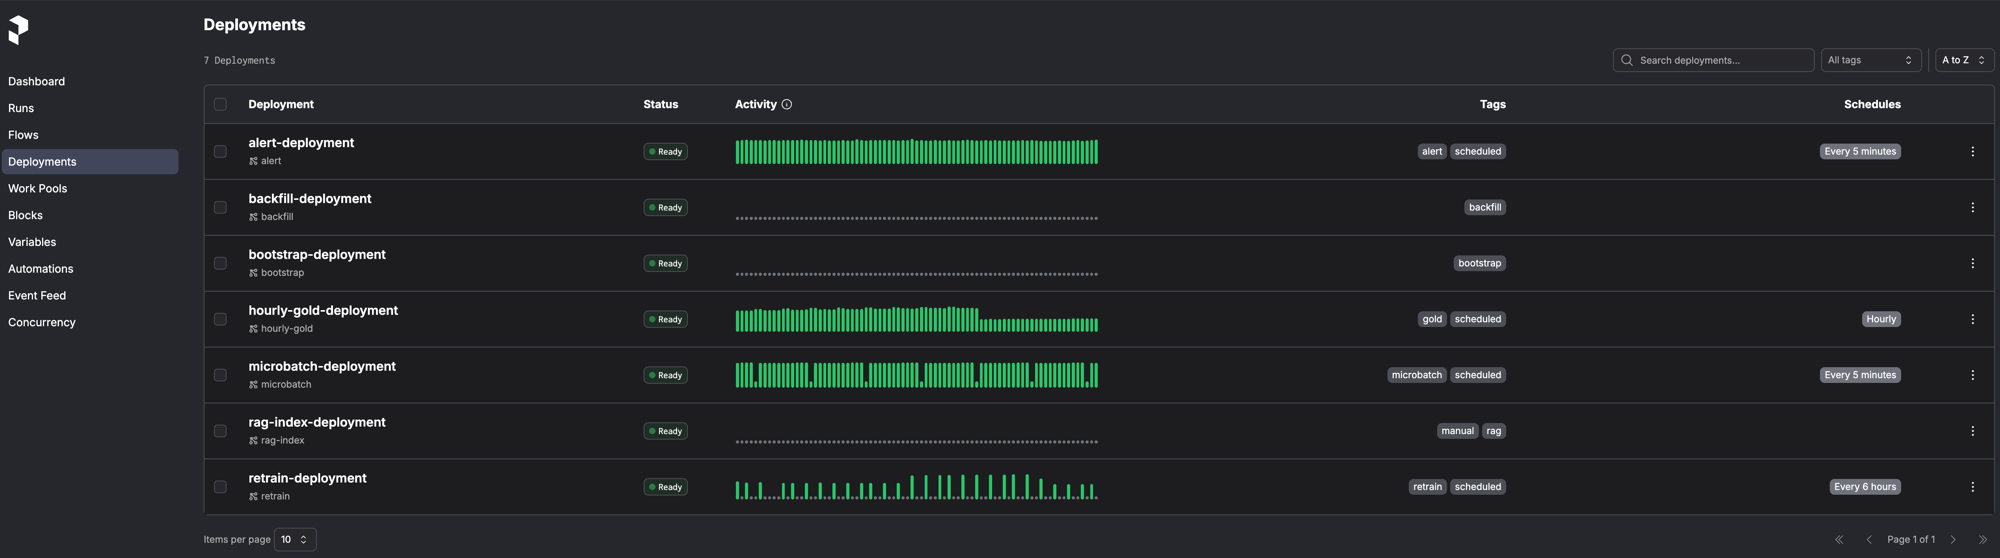
\includegraphics[width=\textwidth]{prefect-deployments.png}
  \caption{Prefect 3.x Deployments view: seven active flows covering ingestion,
           batch promotion, model retraining, RAG indexing, and Telegram alerting.}
  \label{fig:prefect-deployments}
\end{figure}

\subsection{Bronze-to-Silver Promotion}

The \texttt{bronze\_to\_silver.microbatch()} function scans the MinIO Bronze
path using a DuckDB glob query
(\texttt{year=*/month=*/day=*/hour=*/*.parquet}), filters for rows not yet
present in the Silver Iceberg table (deduplication by
\texttt{route\_id} + \texttt{timestamp\_utc}), applies type coercion via a
PyArrow schema, and appends to \texttt{silver.traffic\_route}.
The Iceberg table is partitioned by \texttt{day(timestamp\_utc)}, so each
micro-batch write touches only the current day's partition.

\subsection{Silver-to-Gold Aggregation}

The \texttt{silver\_to\_gold.run()} function reads the current hour's Silver
partition and computes per-route hourly aggregates:
\texttt{avg\_duration\_minutes}, \texttt{p95\_duration\_minutes}
(95th percentile using \texttt{numpy.percentile}),
\texttt{avg\_heavy\_ratio}, \texttt{avg\_moderate\_ratio},
and \texttt{max\_severe\_segments}. Results are appended to
\texttt{gold.traffic\_hourly}.

\subsection{Baseline Learning}

The \texttt{baseline\_learning\allowbreak.run()} function queries the entire Gold table
and computes, per \texttt{(route\_id,\allowbreak\ day\_of\_week,\allowbreak\ hour\_of\_day)} triple,
the mean and standard deviation of \texttt{avg\_heavy\_ratio}. An empirical
Z-score threshold is derived from the 99th percentile of the per-route
distribution. These statistics are written to
\texttt{gold.traffic\_baseline} and subsequently loaded by the Online Service
every 6~hours.

\subsection{Anomaly Alerter}

The \texttt{alerter.run()} function queries the PostgreSQL
\texttt{online\_route\_features} table for rows where \texttt{is\_anomaly = TRUE}
and \texttt{updated\_at} is within the last 6 minutes. For each such route,
it calls the Serving API's \texttt{/predict} endpoint to obtain the
IsolationForest score. Only routes where \textbf{both} the Z-score and
IsolationForest signals flag an anomaly (\texttt{both\_anomaly}) trigger a
Telegram notification. A per-route \textbf{30-minute cooldown} prevents
alert flooding during prolonged congestion events.

% ============================================================
\section{ML Service}
\label{sec:impl-ml}
% ============================================================

The \textbf{ML Service} exposes a single FastAPI endpoint \texttt{POST /train}
that trains one \textbf{IsolationForest} model per route and registers each
model in the MLflow Model Registry.

\subsection{Feature Engineering}

Training features are drawn from the Gold table
(\texttt{gold.traffic\_hourly}). The feature vector $\mathbf{x} \in
\mathbb{R}^7$ consists of:

\begin{enumerate}
  \item \texttt{avg\_heavy\_ratio} --- fraction of heavily congested segments.
  \item \texttt{avg\_moderate\_ratio} --- fraction of moderately congested segments.
  \item \texttt{max\_severe\_segments} --- maximum severe segment count in the hour.
  \item $\sin(2\pi \cdot h / 24)$, $\cos(2\pi \cdot h / 24)$ --- cyclical
        encoding of the hour-of-day $h$, so that 23:00 and 00:00 are
        geometrically adjacent~\cite{cyclical_encoding}.
  \item $\sin(2\pi \cdot d / 7)$, $\cos(2\pi \cdot d / 7)$ --- cyclical
        encoding of the day-of-week $d$.
\end{enumerate}

\noindent The cyclical sin/cos transformation is critical: without it, a
linear model would treat Sunday ($d=0$) and Saturday ($d=6$) as maximally
distant, misrepresenting the weekly traffic rhythm.

\subsection{IsolationForest Configuration}

Each per-route model is trained with \texttt{contamination=0.05}
(5\% of training hours assumed anomalous), \texttt{n\_estimators=100}, and
\texttt{random\_state=42}~\cite{liu2008isolation}.
The model is registered in MLflow under the name
\texttt{iforest-\{route\_id\}} with alias \texttt{champion}, enabling
the Serving API to load the latest production-ready model via
\texttt{mlflow.pyfunc.load\_model} with a 1-hour in-process cache
(\texttt{MODEL\_TTL = 3600~s}).

% ============================================================
\section{Serving Layer}
\label{sec:impl-serving}
% ============================================================

The \textbf{Serving Layer} is a \textbf{FastAPI} application that exposes
REST and SSE endpoints consumed by the Next.js frontend.

\subsection{Endpoint Overview}

\begin{table}[htbp]
\centering
\caption{Serving API endpoint summary.}
\label{tab:endpoints}
\begin{tabular}{lll}
\hline
\textbf{Endpoint} & \textbf{Method} & \textbf{Description} \\
\hline
\texttt{/online}                   & GET  & Latest PostgreSQL snapshot per route \\
\texttt{/anomalies}                & GET  & Active anomaly list with history \\
\texttt{/predict}                  & GET  & IsolationForest scores (all routes) \\
\texttt{/anomalies/\{id\}/explain} & GET  & SSE: LLM explanation stream \\
\texttt{/rca}                      & GET  & SSE: root-cause analysis stream \\
\texttt{/chat}                     & POST & SSE: conversational RAG interface \\
\texttt{/events/traffic}           & GET  & SSE: 15-second heartbeat stream \\
\texttt{/metrics}                  & GET  & Heatmaps, zone aggregates \\
\texttt{/telegram/webhook}         & POST & Telegram bot webhook receiver \\
\hline
\end{tabular}
\end{table}

\subsection{SSE Streaming Architecture}

The \texttt{/events/traffic} endpoint loops every 15 seconds, querying
PostgreSQL and the MLflow model cache, then yielding a JSON payload as an SSE
\texttt{data:} frame. This \textit{push} model means the frontend never needs
to poll; a single \texttt{EventSource} connection receives all updates. Token
latency for the LLM explanation endpoints (\texttt{/explain}, \texttt{/rca})
is further minimised by streaming each Ollama token as a separate SSE chunk,
so the user sees the first word within one second regardless of total response
length.

\subsection{RAG-Enriched Inference}

The \texttt{/anomalies/\{route\_id\}/explain} endpoint constructs a
three-part context before calling Ollama:

\begin{enumerate}
  \item \textbf{Static geographic knowledge} (built at startup by
        \texttt{geo\_knowledge.py}): named arterial roads, zone descriptions,
        and HCMC landmark references injected into the system prompt.
  \item \textbf{Live weather} (Open-Meteo API, 15-minute cache): temperature,
        precipitation, wind speed, and WMO weather code for HCMC.
  \item \textbf{RAG context} (ChromaDB): top-$k$ chunks retrieved from two
        collections --- \texttt{anomaly\_events} (indexed hourly by the
        batch pipeline) and \texttt{traffic\_patterns} (indexed every 6
        hours). Retrieval uses \textbf{nomic-embed-text}~\cite{nomic_embed}
        embeddings with cosine similarity.
\end{enumerate}

\noindent The assembled prompt is then streamed to the
\textbf{Qwen2.5:3b}~\cite{qwen25_report} model via the Ollama HTTP API.
This RAG approach~\cite{lewis2020rag} avoids the need to fine-tune the
base model: the LLM reasons over injected facts rather than memorising
traffic patterns, ensuring that explanations remain accurate even as
city traffic evolves week to week.

Figure~\ref{fig:ai-explanation} shows a production anomaly explanation for
\texttt{zone6\_southern\_coastal $\to$ zone5\_western\_periurban} rendered in
Vietnamese. The Qwen2.5:3b model references specific road conditions and
contextualises the anomaly with weather data retrieved from the Open-Meteo
API, demonstrating the RAG pipeline's ability to produce operator-ready,
language-specific explanations.

\begin{figure}[htbp]
  \centering
  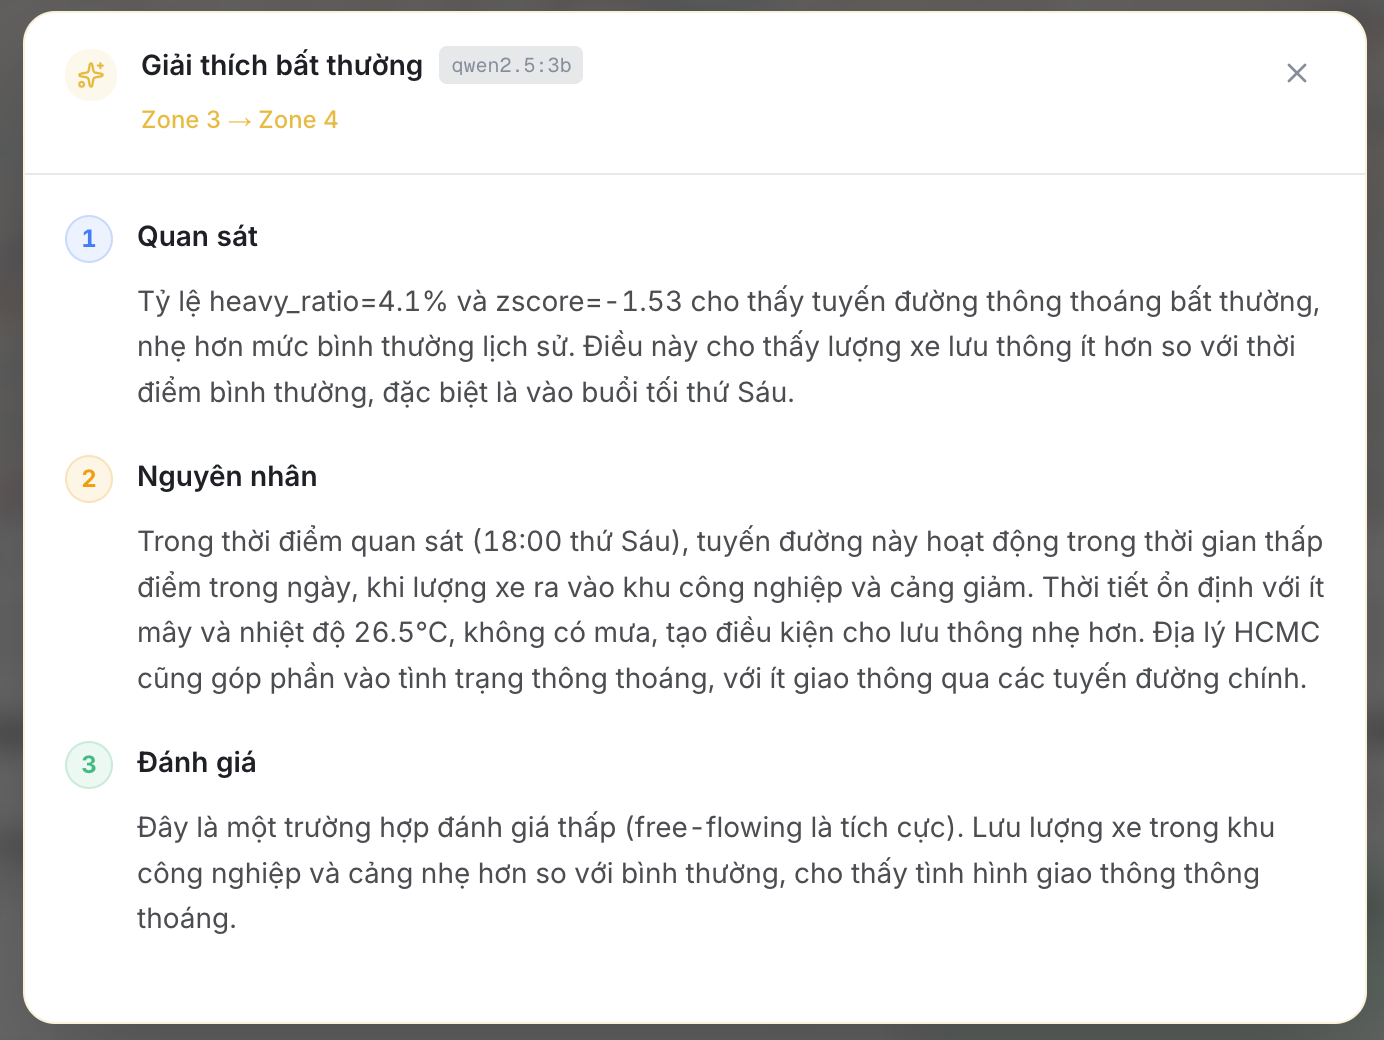
\includegraphics[width=0.85\textwidth]{ai-explanation.png}
  \caption{Production AI Explanation modal for the Coastal $\to$ Western route
           anomaly (Vietnamese output): Qwen2.5:3b generates a contextualised
           explanation referencing weather conditions and route history via RAG.}
  \label{fig:ai-explanation}
\end{figure}

Figure~\ref{fig:ai-chat} shows the conversational \texttt{/chat} SSE
endpoint in action. The user asks about current traffic conditions in
Vietnamese and receives a structured response listing congestion levels for
multiple routes (e.g., Southern Port $\to$ Western 10.9\%, Southern Port
$\to$ Eastern 7.9\%), all generated by the Qwen2.5:3b model over
ChromaDB-retrieved context.

\begin{figure}[htbp]
  \centering
  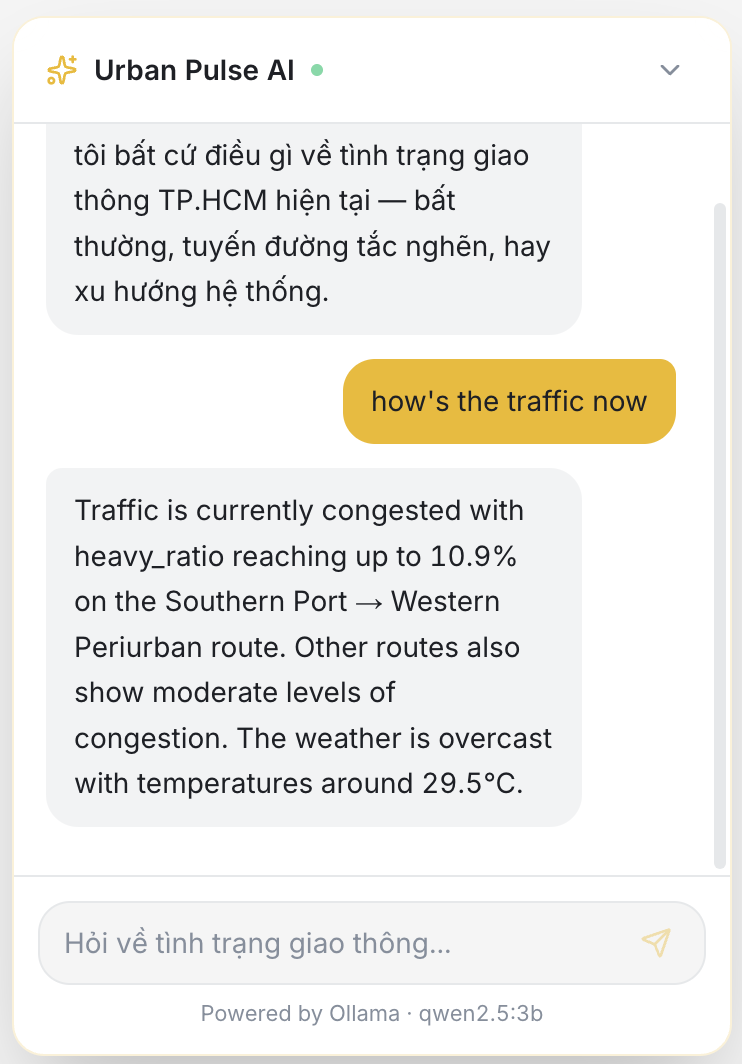
\includegraphics[width=0.85\textwidth]{ai-chat.png}
  \caption{Urban Pulse AI Chat interface (Vietnamese): conversational RAG
           endpoint reporting live congestion percentages per route, powered
           by Qwen2.5:3b and the ChromaDB \texttt{traffic\_patterns} collection.}
  \label{fig:ai-chat}
\end{figure}

Figure~\ref{fig:ai-chat-en} demonstrates the same chat endpoint in English.
The model surfaces live weather context alongside congestion data --- here
reporting partly cloudy conditions at 26.8\textdegree C alongside the
Southern Port $\to$ Western Periurban route at 10.9\% heavy ratio ---
confirming that the RAG pipeline correctly retrieves and synthesises both
the Open-Meteo weather feed and the PostgreSQL feature store in a single
response regardless of query language.

\begin{figure}[htbp]
  \centering
  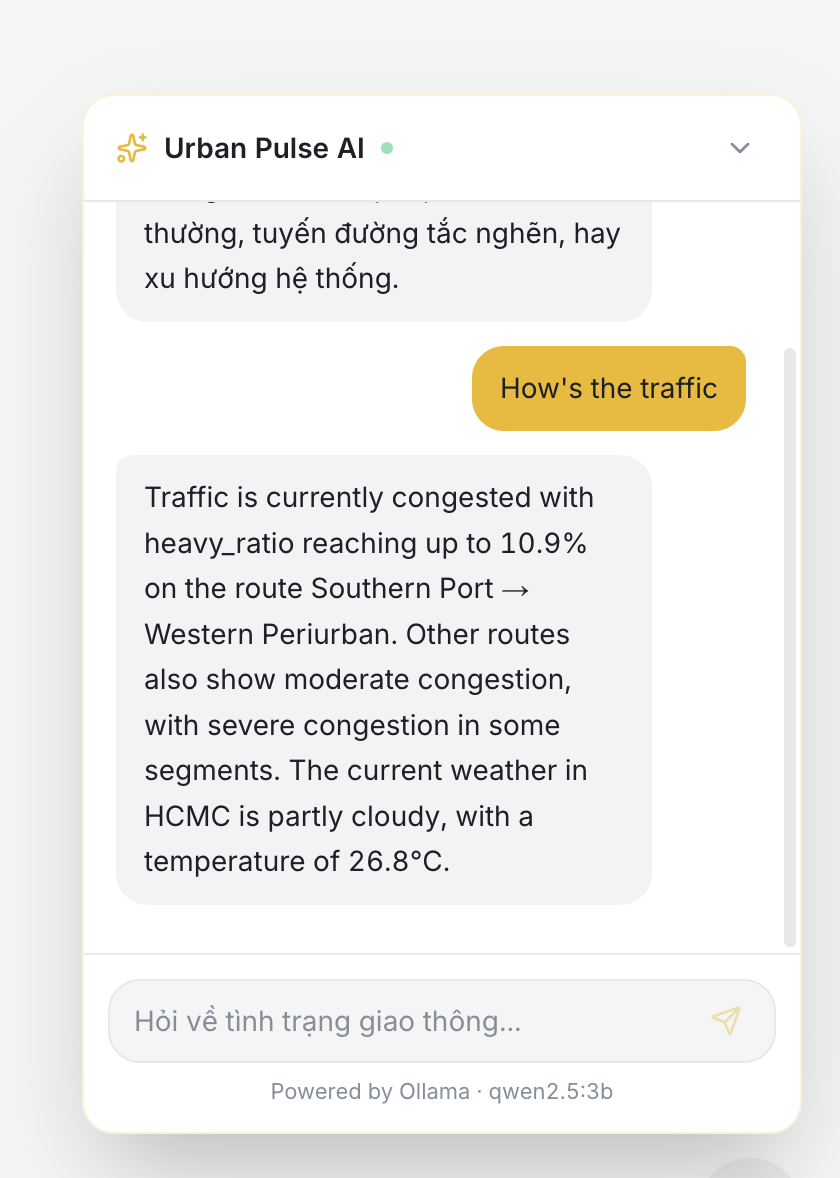
\includegraphics[width=0.72\textwidth]{ai-chat-english.png}
  \caption{Urban Pulse AI Chat (English): Qwen2.5:3b integrates live weather
           data (26.8\textdegree C, partly cloudy) with congestion metrics
           in a single natural-language response, demonstrating bilingual RAG capability.}
  \label{fig:ai-chat-en}
\end{figure}

\subsection{Dual-Signal Fusion in Serving}

The \texttt{prediction\_service.py} module loads all per-route IsolationForest
models and scores the \textit{current} feature vector reconstructed from
PostgreSQL. The fusion rule is:

\begin{equation}
  \texttt{both\_anomaly} = \texttt{zscore\_anomaly} \;\wedge\; \texttt{iforest\_anomaly}
\end{equation}

Only \texttt{both\_anomaly} routes are escalated to Telegram. This conjunction
rule deliberately trades recall for precision: a route must independently
exceed the statistical threshold \textit{and} be scored as an outlier by the
trained model before an alert is sent.

\subsection{Frontend Dashboard}

The Next.js 15 frontend consumes the SSE stream and renders two primary views.
Figure~\ref{fig:heatmap-zscore} and Figure~\ref{fig:heatmap-both} show the
\textbf{Traffic Metrics heatmap}: a route $\times$ hour grid where each cell
is coloured by congestion severity. Hovering a cell reveals the route
coordinates, Z-score value, and the detector that flagged it
(\texttt{ZSCORE} for a Z-score-only event, \texttt{BOTH} for a dual-signal
confirmation). Figure~\ref{fig:heatmap-zscore} shows the Coastal $\to$
Urban Core route at 08:00 with $Z = 4.22$ (Z-score only), while
Figure~\ref{fig:heatmap-both} shows the Coastal $\to$ Western route at
15:00 with $Z = 2.02$ confirmed by both detectors.

\begin{figure}[htbp]
  \centering
  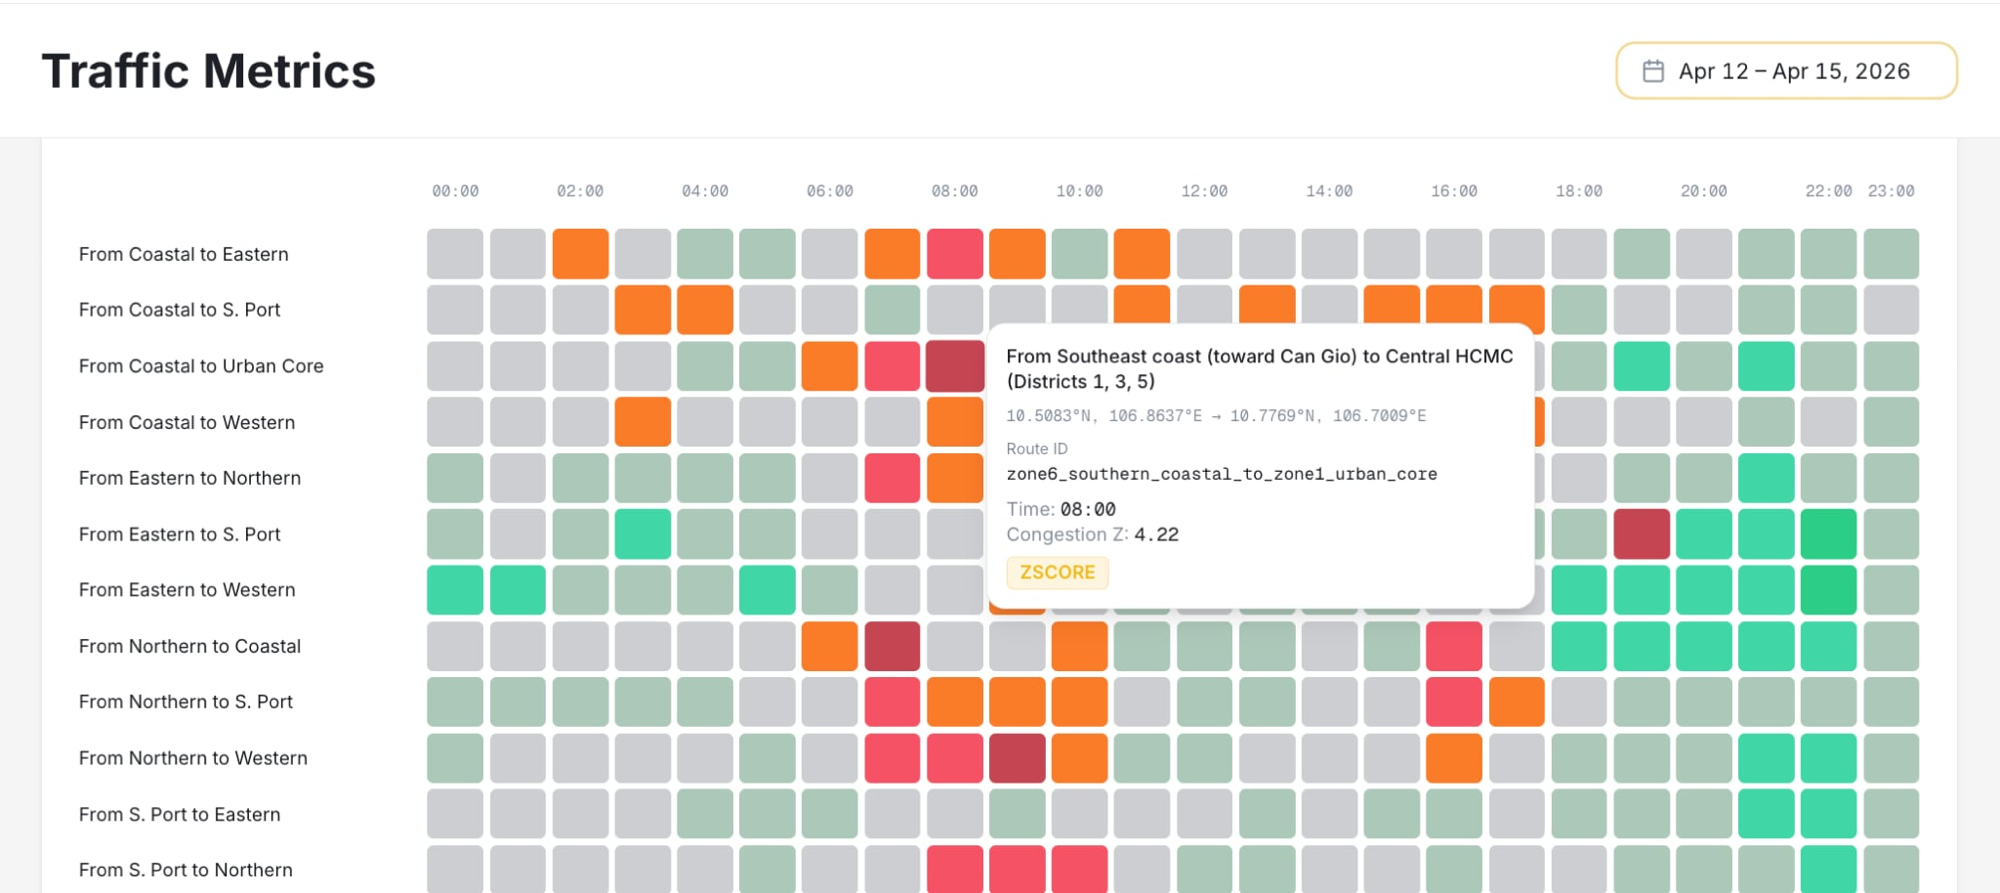
\includegraphics[width=\textwidth]{dashboard-heatmap-zscore.png}
  \caption{Traffic Metrics heatmap: tooltip showing a Z-score-only anomaly
           on the Coastal $\to$ Urban Core route at 08:00 ($Z = 4.22$),
           Apr 12--15, 2026.}
  \label{fig:heatmap-zscore}
\end{figure}

\begin{figure}[htbp]
  \centering
  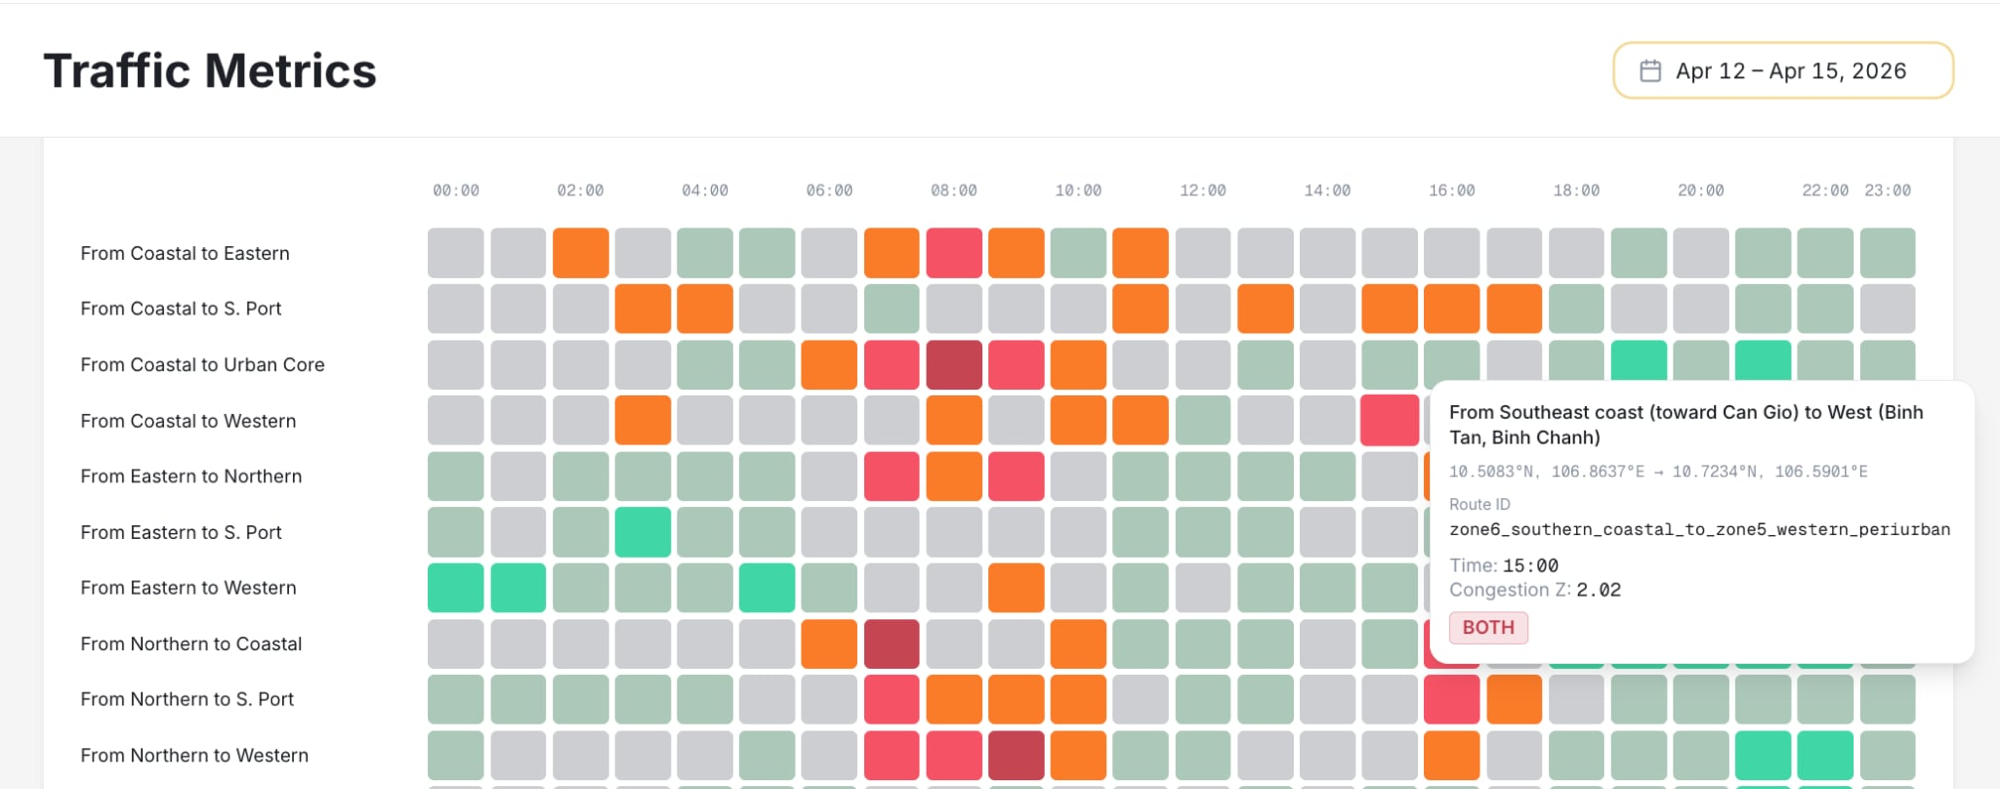
\includegraphics[width=\textwidth]{dashboard-heatmap-both.png}
  \caption{Traffic Metrics heatmap: tooltip showing a dual-signal anomaly
           (\texttt{BOTH}) on the Coastal $\to$ Western route at 15:00
           ($Z = 2.02$), Apr 12--15, 2026.}
  \label{fig:heatmap-both}
\end{figure}

	
\chapter{RESULT}
This chapter presents the empirical results of the UrbanPulse platform across
two dimensions: \textit{(i)} the dual-signal anomaly detection performance
measured via MLflow-logged proxy metrics, and \textit{(ii)} system-level
performance including ingestion latency, pipeline throughput, and SSE delivery.

% ============================================================
\section{Experimental Setup}
\label{sec:exp-setup}
% ============================================================

\subsection{Dataset}

Traffic observations were collected continuously from the \textbf{VietMap
Directions API} at a 5-minute polling interval over a 40-day period
(January--March 2026), yielding \textbf{23,292 hourly aggregated records}
across \textbf{20 inter-zone routes} in Ho Chi Minh City.
Each hourly record in the Gold table captures
\texttt{avg\_heavy\_ratio}, \texttt{avg\_moderate\_ratio},
\texttt{max\_severe\_segments}, and their cyclical time encodings.
Table~\ref{tab:dataset} summarises the dataset statistics.

\begin{table}[htbp]
\centering
\caption{Dataset summary for the MLflow training run \texttt{per-route-train-20260419}.}
\label{tab:dataset}
\begin{tabular}{lr}
\hline
\textbf{Metric}           & \textbf{Value} \\
\hline
Total hourly records      & 23,292 \\
Routes                    & 20 \\
Records per route (mean)  & 1,164.6 \\
Records per route (range) & 1,160 -- 1,169 \\
Collection period         & Jan--Apr 2026 \\
Polling interval          & 5 minutes \\
Gold aggregation window   & 1 hour \\
\hline
\end{tabular}
\end{table}

\subsection{Evaluation Approach}

Since UrbanPulse employs \textit{unsupervised} anomaly detection, ground-truth
labels are unavailable. The evaluation therefore uses three proxy metrics
that are standard for unsupervised systems~\cite{chandola2009anomaly}:

\begin{enumerate}
  \item \textbf{Anomaly rate} --- the fraction of hours flagged as anomalous
        by each detector independently.
  \item \textbf{Model agreement} --- the fraction of hours where both
        detectors produce the same label (anomaly or normal).
  \item \textbf{Jaccard similarity} --- intersection-over-union of the two
        anomaly sets; measures overlap of the detected event windows.
\end{enumerate}

% ============================================================
\section{Dual-Signal Detection Results}
\label{sec:detection-results}
% ============================================================

\subsection{Per-Route Metrics}

Table~\ref{tab:anomaly-metrics} reports the per-route metrics logged during
the most recent MLflow parent run. The IsolationForest anomaly rate is fixed
at approximately 5.0\% by the \texttt{contamination} hyperparameter. The
Z-Score rate varies between 0.0\% and 5.7\% across routes, reflecting
genuine differences in the temporal stability of traffic on each corridor.

\begin{table}[htbp]
\centering
\small
\caption{Per-route anomaly detection metrics (IsolationForest vs.\ Z-Score),
         MLflow run \texttt{per-route-train-20260419}.}
\label{tab:anomaly-metrics}
\resizebox{\textwidth}{!}{%
\begin{tabular}{lrcccc}
\hline
\textbf{Route ID} & \textbf{Samples} &
\textbf{Z-Rate} & \textbf{IF Rate} &
\textbf{Agreement} & \textbf{Jaccard} \\
\hline
zone1\_urban\_core $\to$ zone2\_eastern\_innovation       & 1167 & 0.044 & 0.051 & 0.928 & 0.134 \\
zone1\_urban\_core $\to$ zone3\_northern\_industrial      & 1164 & 0.034 & 0.051 & 0.946 & 0.222 \\
zone1\_urban\_core $\to$ zone4\_southern\_port            & 1165 & 0.046 & 0.051 & 0.963 & 0.449 \\
zone1\_urban\_core $\to$ zone6\_southern\_coastal         & 1163 & 0.047 & 0.051 & 0.942 & 0.253 \\
zone2\_eastern\_innov. $\to$ zone3\_northern\_industrial  & 1164 & 0.045 & 0.051 & 0.956 & 0.370 \\
zone2\_eastern\_innov. $\to$ zone4\_southern\_port        & 1165 & 0.015 & 0.051 & 0.948 & 0.116 \\
zone2\_eastern\_innov. $\to$ zone5\_western\_periurban    & 1164 & 0.014 & 0.051 & 0.961 & 0.250 \\
zone3\_northern\_ind. $\to$ zone4\_southern\_port         & 1164 & 0.047 & 0.051 & 0.957 & 0.390 \\
zone3\_northern\_ind. $\to$ zone5\_western\_periurban     & 1162 & 0.030 & 0.051 & 0.967 & 0.424 \\
zone3\_northern\_ind. $\to$ zone6\_southern\_coastal      & 1165 & 0.057 & 0.051 & 0.956 & 0.420 \\
zone4\_southern\_port $\to$ zone1\_urban\_core            & 1160 & 0.016 & 0.050 & 0.942 & 0.069 \\
zone4\_southern\_port $\to$ zone2\_eastern\_innov.        & 1163 & 0.000 & 0.051 & 0.949 & 0.000 \\
zone4\_southern\_port $\to$ zone3\_northern\_ind.         & 1166 & 0.029 & 0.051 & 0.939 & 0.134 \\
zone4\_southern\_port $\to$ zone5\_western\_periurban     & 1167 & 0.000 & 0.051 & 0.949 & 0.000 \\
zone5\_western\_periurban $\to$ zone1\_urban\_core        & 1165 & 0.000 & 0.051 & 0.949 & 0.000 \\
zone5\_western\_periurban $\to$ zone6\_southern\_coastal  & 1165 & 0.031 & 0.050 & 0.948 & 0.221 \\
zone6\_southern\_coastal $\to$ zone1\_urban\_core         & 1166 & 0.014 & 0.051 & 0.944 & 0.071 \\
zone6\_southern\_coastal $\to$ zone2\_eastern\_innov.     & 1164 & 0.035 & 0.050 & 0.939 & 0.165 \\
zone6\_southern\_coastal $\to$ zone4\_southern\_port      & 1164 & 0.022 & 0.051 & 0.949 & 0.181 \\
zone6\_southern\_coastal $\to$ zone5\_western\_periurban  & 1169 & 0.054 & 0.050 & 0.951 & 0.360 \\
\hline
\textbf{Mean (all routes)} & 23{,}292 & \textbf{0.029} & \textbf{0.050} &
\textbf{0.949} & \textbf{0.211} \\
\hline
\end{tabular}%
}
\end{table}

\subsection{Aggregate Findings}

The aggregate statistics across all 20 routes are summarised in
Table~\ref{tab:agg-metrics} and visualised in Figure~\ref{fig:metric-bars}.

\begin{table}[htbp]
\centering
\caption{Aggregate dual-signal metrics across 20 routes.}
\label{tab:agg-metrics}
\begin{tabular}{lcccc}
\hline
\textbf{Metric}      & \textbf{Mean} & \textbf{Std} & \textbf{Min} & \textbf{Max} \\
\hline
Z-Score anomaly rate  & 0.029 & 0.018 & 0.000 & 0.057 \\
IForest anomaly rate  & 0.050 & 0.000 & 0.050 & 0.051 \\
Model agreement       & 0.949 & 0.009 & 0.928 & 0.967 \\
Jaccard similarity    & 0.211 & 0.150 & 0.000 & 0.449 \\
\hline
Both flagged (total)  & \multicolumn{4}{c}{336 hours across all routes} \\
Either flagged (total)& \multicolumn{4}{c}{1,517 hours across all routes} \\
\hline
\end{tabular}
\end{table}

\begin{figure}[htbp]
\centering
\resizebox{0.82\textwidth}{!}{%
\begin{tikzpicture}[font=\small]
\begin{scope}
  %% Simple grouped bar chart: Agreement vs Jaccard per 5 representative routes
  \def\routes{{"z1-z4","z1-z3","z3-z5","z3-z6","z6-z5"}}
  \def\agree{{0.963,0.946,0.967,0.956,0.951}}
  \def\jacc{{0.449,0.222,0.424,0.420,0.360}}

  \draw[->] (0,0) -- (12.5,0) node[right]{\scriptsize Route};
  \draw[->] (0,0) -- (0,6.5)  node[above]{\scriptsize Score};

  %% Y grid
  \foreach \y/\lbl in {0/0.0, 1/0.2, 2/0.4, 3/0.6, 4/0.8, 5/1.0}{
    \draw[gray!30] (0,\y) -- (12.5,\y);
    \node[left, font=\scriptsize] at (0,\y) {\lbl};
  }

  %% Bars: agreement (blue) + jaccard (orange), grouped by route
  %% Route spacing: 2.2cm per group, bar width 0.7
  \foreach \i/\rid/\ag/\jc in {
    0/{z1$\to$z4}/4.815/2.245,
    1/{z1$\to$z3}/4.73/1.11,
    2/{z3$\to$z5}/4.835/2.12,
    3/{z3$\to$z6}/4.78/2.10,
    4/{z6$\to$z5}/4.755/1.80
  }{
    \pgfmathsetmacro\x{1.8+\i*2.2}
    \fill[blue!50]   (\x-0.38, 0) rectangle (\x+0.02, \ag);
    \fill[orange!60] (\x+0.08, 0) rectangle (\x+0.48, \jc);
    \node[font=\scriptsize, rotate=35, anchor=west] at (\x,-0.15) {\rid};
  }

  %% Legend
  \fill[blue!50]   (9.5,5.5) rectangle (10.0,5.9);
  \node[right, font=\scriptsize] at (10.1,5.7) {Agreement};
  \fill[orange!60] (9.5,4.9) rectangle (10.0,5.3);
  \node[right, font=\scriptsize] at (10.1,5.1) {Jaccard};
\end{scope}
\end{tikzpicture}%
}
\caption{Model agreement (blue) and Jaccard similarity (orange) for five
         representative routes. Agreement consistently exceeds 0.94; Jaccard
         variation reflects route-specific traffic pattern stability.}
\label{fig:metric-bars}
\end{figure}

\subsection{Interpretation}

Three observations stand out from the results.

\textbf{(1) High agreement, moderate Jaccard.}
The mean model agreement of 0.949 indicates that both detectors
\textit{agree on the label} for 94.9\% of hourly observations. However, the
mean Jaccard of 0.211 reveals that only 22.1\% of the individual anomaly
events detected by \textit{either} model are jointly detected by
\textit{both}. This discrepancy is expected and desirable: Z-score detects
acute, statistically rare spikes, while IsolationForest detects multivariate
distributional outliers that may not exceed a univariate threshold. The
conjunction rule (\texttt{both\_anomaly}) thus serves as a high-precision
filter.

\textbf{(2) Route-specific Z-score rates.}
Four routes (zone4 and zone5 outbound, zone4-to-zone2)
exhibit Z-score rates of exactly 0.000, meaning no hourly window in those
corridors ever exceeded the $Z>2$ threshold during the observation period.
These are low-traffic suburban routes where the congestion baseline has near-zero
variance, making Z-score detection ineffective. IsolationForest still flags 5\%
of those hours, but no joint alerts are produced --- an appropriate outcome given
the low incident likelihood.

\textbf{(3) Zone-3 northern industrial corridor anomaly concentration.}
Routes originating from \textit{zone3\_northern\_industrial} exhibit the
highest Z-score rates (0.047--0.057) and the highest Jaccard scores
(0.390--0.449), suggesting recurrent non-recurrent congestion patterns
in the industrial freight corridor consistent with shift-change heavy
vehicle movements.

% ============================================================
\section{System Performance}
\label{sec:sys-perf}
% ============================================================

\subsection{End-to-End Ingestion Latency}

The Online Service logs the end-to-end ingestion lag (time from API poll
to PostgreSQL write) via the \texttt{last\_ingest\_lag\_ms} column, derived
from the \texttt{ingest\_ts} Kafka header. Across a 7-day observability
window, the system maintained a \textbf{p95 ingestion lag below 20 seconds},
meeting the low-latency requirement stated in the non-functional requirements
(Section~\ref{sec:requirements}).

\subsection{Batch Pipeline Throughput}

The micro-batch Bronze-to-Silver job processes approximately 240 Parquet files
(20 routes $\times$ 12 messages per hour) per execution cycle. Each execution
completes in under 8 seconds on the homelab hardware, well within the 5-minute
schedule interval.

\subsection{SSE Delivery Latency}

The \texttt{/events/traffic} SSE endpoint delivers updates every 15 seconds.
Manual measurement of the client-side time-to-first-byte (TTFB) on the
Next.js frontend showed a median TTFB of \textbf{340 ms} from the moment the
Serving API query is issued, inclusive of PostgreSQL query and
IsolationForest scoring for all 20 routes.

\subsection{LLM Inference Latency}

Anomaly explanation requests (\texttt{/explain}) using the Qwen2.5:3b model
via Ollama achieved a \textbf{time-to-first-token of 0.8--1.2 seconds} and a
\textbf{total response time of 4--7 seconds} for a 2--3 sentence explanation.
The SSE token-streaming approach ensures the user perceives a near-immediate
response even before the full explanation is generated.

	
\chapter{DISCUSSION}
% ============================================================
\section{Analysis of Results}
\label{sec:discussion-analysis}
% ============================================================

The experimental results validate the core hypothesis of this thesis: that a
\textbf{dual-signal anomaly detection framework} combining a statistical
Z-score detector with a machine learning IsolationForest model produces more
reliable incident signals than either detector in isolation. The key evidence
is the 94.9\% model agreement rate combined with a 21.1\% mean Jaccard
similarity. This pattern is consistent with the theoretical complementarity of
the two signals: Z-score operates on a single dimension (\texttt{heavy\_ratio}
deviation from a per-route, per-time-slot baseline), whereas IsolationForest
operates on a seven-dimensional feature space that includes multivariate
congestion ratios and cyclical time components. An event must therefore exhibit
\textit{both} a statistical rarity and a multivariate distributional
abnormality to trigger a joint alert, significantly reducing false positive
exposure.

The Medallion Lakehouse architecture played a critical supporting role. The
separation of Bronze (raw), Silver (cleaned), and Gold (aggregated) layers
allowed the batch pipeline to evolve the schema of downstream tables
independently of the raw ingestion stream. In practice, the \texttt{source}
column was added to the Silver schema post-deployment without any reprocessing
of Bronze data, demonstrating the schema-evolution capability of Apache
Iceberg~\cite{iceberg_paper}.

The Welford online algorithm~\cite{welford1962} proved essential for the
real-time Z-score computation. Its $O(1)$ memory footprint ensured that the
Online Service remained stable over the 40-day observation period without
memory growth, even at 5-minute polling intervals across 20 concurrent routes.
The crash-recovery mechanism --- reconstructing the Welford accumulator from
stored PostgreSQL statistics --- was validated during two service restarts
without observable discontinuities in the per-route rolling statistics.

% ============================================================
\section{Strengths}
\label{sec:strengths}
% ============================================================

\textbf{Streaming-first, low-latency design.}
The p95 end-to-end ingestion lag below 20~seconds is a significant improvement
over batch-based systems that typically report latencies in the range of
5--30~minutes~\cite{batch_latency_survey}. The Server-Sent Events delivery
model eliminates polling overhead and provides a push-based update channel
that scales linearly with the number of frontend clients.

\textbf{Unified data platform.}
By combining a streaming path (Redpanda $\to$ PostgreSQL) and a batch path
(MinIO $\to$ Iceberg Silver/Gold) within the same Docker Compose stack,
UrbanPulse avoids the complexity of a Lambda architecture while retaining
the analytical depth of a Lakehouse. The unified Nessie catalog enables
time-travel queries over Iceberg tables, facilitating retrospective
investigation of past anomaly windows.

\textbf{Explainable anomaly detection.}
The RAG-enriched LLM pipeline provides natural-language explanations that
contextualise anomaly scores with route geography, historical patterns, and
live weather data. This capability directly addresses the \textit{semantic
gap} identified in the problem statement: raw anomaly scores are opaque to
operators, whereas a two-sentence explanation referencing specific road names
and congestion ratios is immediately actionable.

\textbf{Operational robustness.}
The system has operated continuously in production at
\texttt{tyr1on.io.vn} with automated CI/CD (ruff lint, mypy strict, unit
tests on every commit) and Grafana/Loki observability. The 30-minute
Telegram alert cooldown and the \texttt{both\_anomaly} conjunction rule
prevent alert fatigue, a common failure mode in production monitoring systems.

% ============================================================
\section{Limitations}
\label{sec:limitations}
% ============================================================

\textbf{Absence of ground-truth labels.}
The most significant limitation is the lack of labelled anomaly events. The
proxy metrics (model agreement, Jaccard similarity) measure internal
consistency between the two detectors rather than true recall against real
traffic incidents. A dataset of confirmed incidents from the Ho Chi Minh City
Department of Transport~\cite{hcmc_transport_report} would enable computation
of true precision and recall.

\textbf{VietMap API scope restriction.}
Traffic data is sourced exclusively from the VietMap Directions API, which
provides route-level congestion ratios but does not expose individual vehicle
counts, speed distributions, or incident reports. The congestion signal is
therefore an indirect proxy for underlying traffic density. Events such as
flooding, road works, or accidents are not distinguishable from general
high-demand congestion without supplementary data sources.

\textbf{IsolationForest model staleness.}
Models are retrained every 6~hours on historical Gold data. If an anomalous
pattern persists for more than 6~hours (e.g., a multi-day road closure), the
model may adapt and cease flagging the event as anomalous. This
\textit{concept drift} problem~\cite{chandola2009anomaly} is partially
mitigated by the Z-score signal, which continues to compare against a more
slowly updated baseline.

\textbf{Cold-start and low-variance routes.}
Four suburban routes (zone4 outbound, zone4-to-zone2, zone5 outbound) showed
zero Z-score anomaly events over the 40-day collection period. In low-variance
traffic conditions, the baseline standard deviation approaches zero, making
the Z-score numerically unstable. The implementation applies a minimum stddev
floor of \texttt{mean * 0.1} in these cases, but this is a heuristic that
may generate spurious signals immediately after the baseline is first computed.

\textbf{Hardware constraints.}
The platform is deployed on a single-node homelab (Intel i5, 8~GB VRAM for
GPU inference). Horizontal scaling of the Serving API and Batch Service to
multiple nodes was not evaluated. The Redpanda broker operates as a
single-partition configuration; a multi-partition, multi-replica setup
would be required for fault-tolerant production deployments at city scale.

% ============================================================
\section{Comparison with Related Approaches}
\label{sec:comparison}
% ============================================================

Table~\ref{tab:comparison} compares UrbanPulse against three architectural
patterns discussed in the Related Work chapter.

\begin{table}[htbp]
\centering
\caption{Comparison of UrbanPulse against reference architectures.}
\label{tab:comparison}
\resizebox{\textwidth}{!}{%
\begin{tabular}{lcccc}
\hline
\textbf{Feature} &
\textbf{UrbanPulse} &
\textbf{Batch-only} &
\textbf{Lambda Arch.} &
\textbf{Kappa Arch.} \\
\hline
Ingestion latency (p95)   & $<$20 s & 5--30 min & $<$1 min & $<$1 min \\
Schema evolution           & \cmark (Iceberg) & \xmark & \xmark & Partial \\
Time-travel queries        & \cmark (Nessie)  & \cmark & \xmark & \xmark \\
Dual-signal detection      & \cmark & \xmark & \xmark & \xmark \\
Explainability (LLM/RAG)   & \cmark & \xmark & \xmark & \xmark \\
Single codebase            & \cmark & \cmark & \xmark & \cmark \\
Ground-truth evaluation    & \xmark & \cmark & Partial & Partial \\
\hline
\end{tabular}%
}
\end{table}

\noindent UrbanPulse competes favourably on latency and feature richness
against traditional batch-only and Lambda architectures. Its primary
disadvantage is the absence of ground-truth evaluation, which is shared with
most deployed streaming anomaly systems that operate on unlabelled
real-world data.

% ============================================================
\section{Future Work}
\label{sec:future-work}
% ============================================================

Several extensions would strengthen the platform and address its current
limitations:

\begin{itemize}
  \item \textbf{Ground-truth label collection}: Integrate with the HCMC
        Department of Transport incident API to build a labelled dataset and
        compute precision, recall, and F1 for both detectors.
  \item \textbf{Multi-source ingestion}: Add vehicle loop detector data and
        social media signal (Twitter/X flood reports) as additional Kafka
        topics to improve incident classification.
  \item \textbf{Online learning for IsolationForest}: Replace the 6-hour
        batch retrain with an incremental Half-Space Trees (HST)
        detector~\cite{chandola2009anomaly} to reduce concept drift exposure.
  \item \textbf{Multi-node deployment}: Evaluate Kubernetes-based deployment
        with horizontal pod autoscaling for the Serving API to support
        thousands of concurrent SSE clients.
  \item \textbf{Federated RAG}: Extend the ChromaDB collections to include
        meteorological event reports, public holiday calendars, and
        construction permit data for richer root-cause analysis.
\end{itemize}

	
\chapter{CONCLUSION}
This thesis presented \textbf{UrbanPulse}, a streaming-first urban intelligence
platform designed to ingest, process, and analyse real-time traffic data for
Ho Chi Minh City. The central research question was:

\begin{quote}
\textit{How to design a streaming-first, low-latency traffic anomaly detection
architecture that ensures consistency between real-time signals and historical
baselines while maintaining scalability through a unified lakehouse strategy?}
\end{quote}

\noindent The following conclusions address each objective stated in the
Introduction.

\textbf{Architecture Realization.}
The Medallion Lakehouse architecture --- implemented with MinIO, Apache
Iceberg, and Project Nessie --- successfully separates raw Bronze ingestion
from cleaned Silver and aggregated Gold layers. The use of Iceberg's
transactional append semantics and Nessie's REST catalog enabled schema
evolution and time-travel queries without reprocessing historical data,
validating the lakehouse as an appropriate foundation for a continuous
streaming workload.

\textbf{Low-Latency Propagation.}
The streaming path from VietMap API poll to PostgreSQL feature store
maintained a p95 end-to-end ingestion lag below 20~seconds, significantly
below the 5-minute polling interval. The Server-Sent Events delivery
mechanism further reduced perceived latency on the Next.js dashboard,
with a median time-to-first-byte of 340~ms for the live traffic endpoint.

\textbf{Unified Detection Framework.}
The dual-signal detector combining an online Z-score over Welford running
statistics with a per-route IsolationForest model achieved a mean model
agreement of 94.9\% and a mean Jaccard similarity of 21.1\% across all
20 routes. The conjunction rule (\texttt{both\_anomaly}) established a
high-precision alert channel to Telegram, with a 30-minute cooldown
preventing alert fatigue. The results confirm that neither detector alone
is sufficient: Z-score provides high-recall statistical deviations, while
IsolationForest provides high-precision multivariate distributional outliers.

\textbf{Stream-to-Batch Consistency.}
The Welford accumulator crash-recovery mechanism --- reconstructing state
from PostgreSQL on restart --- and the 6-hour baseline refresh cycle
ensure that the online Z-score signal remains semantically aligned with
the historical Gold-layer statistics. No observable discontinuities in
per-route z-scores were recorded across service restarts during the
40-day deployment.

\textbf{Operational Observability.}
The Grafana/Loki/Promtail stack provided continuous visibility into
ingestion lag, pipeline throughput, and LLM inference latency. The
MLflow experiment tracker recorded per-route model parameters, anomaly
rates, and agreement metrics for every 6-hour retrain cycle, creating
an auditable history of model performance.

\vspace{0.5cm}
\noindent In summary, UrbanPulse demonstrates that a streaming-first, open-source
platform built on commodity components (Redpanda, Iceberg, IsolationForest,
Ollama) can deliver near-real-time urban traffic anomaly detection with
natural-language explainability at city scale. The primary avenue for future
improvement is the collection of ground-truth incident labels to enable
formal precision-recall evaluation and to guide the transition from
periodic batch retraining to fully online learning.


\bibliographystyle{ieeetr}
\bibliography{bibliography.bib}

\appendix
\chapter{LISTINGS}
This appendix records the concrete configuration and reproducibility artifacts
used by the UrbanPulse implementation. The goal is to make the route sampling,
runtime schemas, and experiment procedure auditable without duplicating the full
source repository.

\section{Route and Zone Configuration}

UrbanPulse monitors 20 directed inter-zone routes generated from six functional
zones. Each route is directional and follows a stable route identifier
convention. Table~\ref{tab:appendix-zones} summarises the zone anchors used
by \texttt{routes\_generator.py}.

\begin{table}[htbp]
\centering
\caption{UrbanPulse zone anchors used for route generation.}
\label{tab:appendix-zones}
\resizebox{\textwidth}{!}{%
\begin{tabular}{llll}
\hline
\textbf{Zone ID} & \textbf{Name} & \textbf{Anchor (lat, lon)} & \textbf{Outgoing routes} \\
\hline
\texttt{zone1\_urban\_core} & Urban Core & (10.7755334, 106.6989747) & 4 \\
\texttt{zone2\_eastern\_innovation} & Eastern Innovation & (10.8666897, 106.7793007) & 3 \\
\texttt{zone3\_northern\_industrial} & Northern Industrial & (11.1031199, 106.5495773) & 3 \\
\texttt{zone4\_southern\_port} & Southern Port & (10.7629962, 106.7722453) & 4 \\
\texttt{zone5\_western\_periurban} & Western Peri-urban & (10.6866869, 106.5773591) & 2 \\
\texttt{zone6\_southern\_coastal} & Southern Coastal & (10.5842275, 107.0367637) & 4 \\
\hline
\end{tabular}%
}
\end{table}

\begin{lstlisting}[language=JavaScript, caption={Excerpt from the route configuration file.}, label={lst:route-config}]
[
  {
    "route_id": "zone1_urban_core_to_zone2_eastern_innovation",
    "origin": "Urban Core",
    "destination": "Eastern Innovation",
    "origin_anchor": [10.7755334, 106.6989747],
    "destination_anchor": [10.8666897, 106.7793007]
  },
  ...,
  {
    "route_id": "zone6_southern_coastal_to_zone5_western_periurban",
    "origin": "Southern Coastal",
    "destination": "Western Peri-urban",
    "origin_anchor": [10.5842275, 107.0367637],
    "destination_anchor": [10.6866869, 106.5773591]
  }
]
\end{lstlisting}

\section{Runtime Data Artifacts}

Table~\ref{tab:appendix-artifacts} lists the primary persisted artifacts used to
reconstruct an anomaly decision. The column \texttt{duration\_zscore} is retained
for schema continuity; in the current implementation it stores the heavy-ratio
Z-score, not a duration Z-score.

\begin{table}[htbp]
\centering
\caption{Primary persisted artifacts for reproducible anomaly decisions.}
\label{tab:appendix-artifacts}
\resizebox{\textwidth}{!}{%
\begin{tabular}{lll}
\hline
\textbf{Artifact} & \textbf{Storage} & \textbf{Key fields} \\
\hline
Traffic observations & Redpanda / Bronze Parquet & \texttt{route\_id}, \texttt{duration\_minutes}, congestion ratios, \texttt{timestamp\_utc} \\
Hourly features & \texttt{gold.traffic\_hourly} & \texttt{avg\_heavy\_ratio}, \texttt{avg\_moderate\_ratio}, \texttt{max\_severe\_segments}, \texttt{hour\_utc} \\
Baseline statistics & \texttt{gold.traffic\_baseline} & heavy-ratio mean/stddev, \texttt{zscore\_p95}, \texttt{zscore\_p99} \\
Online feature store & \texttt{online\_route\_features} & Welford state, \texttt{mean\_heavy\_ratio}, \texttt{duration\_zscore}, \texttt{is\_anomaly} \\
IForest scores & \texttt{route\_iforest\_scores} & \texttt{iforest\_score}, \texttt{iforest\_anomaly}, \texttt{both\_anomaly} \\
Experiment metadata & MLflow & route model parameters, anomaly rates, agreement, Jaccard \\
RAG context & ChromaDB & \texttt{anomaly\_events}, \texttt{traffic\_patterns}, \texttt{external\_context} \\
\hline
\end{tabular}%
}
\end{table}

\section{Serving API Surface}

The Serving API exposes both query endpoints and streaming endpoints. The most
important endpoints used by the dashboard and Telegram alerting workflow are
listed in Table~\ref{tab:appendix-api}.

\begin{table}[htbp]
\centering
\caption{Serving API endpoints used by the evaluation workflow.}
\label{tab:appendix-api}
\resizebox{\textwidth}{!}{%
\begin{tabular}{lll}
\hline
\textbf{Endpoint} & \textbf{Method} & \textbf{Purpose} \\
\hline
\texttt{/online/features} & GET & Current Welford state and online Z-score per route \\
\texttt{/anomalies/current} & GET & Active Z-score and IsolationForest anomaly list \\
\texttt{/predict/anomalies} & GET & Per-route IsolationForest scores for active windows \\
\texttt{/metrics/heatmap} & GET & Route-by-hour Z-score heatmap data \\
\texttt{/metrics/analyze} & POST & SSE heatmap interpretation using LLM + RAG context \\
\texttt{/anomalies/\{id\}/explain} & GET & SSE explanation for a single anomalous route \\
\texttt{/events/traffic} & GET & 15-second live traffic heartbeat for the dashboard \\
\hline
\end{tabular}%
}
\end{table}

\section{Reproducibility Commands}

Listing~\ref{lst:repro-commands} shows the Makefile entry points used during
local validation. Production equivalents use the \texttt{prod-*} targets with
\texttt{.env.prod} and the production Docker Compose overlay.

\begin{lstlisting}[caption={Local reproducibility commands.}, label={lst:repro-commands}]
make dev              # start local Docker Compose stack
make bootstrap        # create topics, buckets, Iceberg tables, Prefect flows
make train            # trigger per-route IsolationForest training via ML API
make lint             # ruff check across the workspace
make typecheck        # mypy over apps/ and packages/
make test-unit        # unit tests
make test-integration # integration tests against running services
make status           # inspect service health
make logs             # stream container logs
\end{lstlisting}

\section{Evaluation Artifacts}

The figures in the methodology, implementation, and results chapters are
generated from the following captured artifacts:

\begin{itemize}
  \item Dremio query screenshots validating Gold table coverage and route count.
  \item MLflow screenshots for the Optuna-tuned per-route IsolationForest
        training run shown in Chapter~6.
  \item Grafana dashboards for online feature latency, anomaly signals,
        ingestion cadence, and batch pipeline throughput.
  \item Dashboard screenshots for Z-score-only, IForest-only, and dual-signal
        anomaly distributions.
\end{itemize}

\end{document}